
%%% Uncomment for slide version
\documentclass{beamer}
\setbeameroption{hide notes} % Only slides

%%% Uncomment for handout version
%\documentclass[handout]{beamer}
%\setbeameroption{show notes on second screen=right} % Both

\usepackage{enumitem}
\usepackage{listings}
\usepackage{adjustbox} % To incorporate code into Latex
\usepackage{multirow} % To merge multiple rows  in a table
\usepackage{soul} % To put in strikethrough text
\usepackage{array}
\usepackage{makecell}

\setbeamertemplate{note page}{\pagecolor{white}\insertnote}
\setbeamertemplate{footline}{}
\usetheme[progressbar=frametitle]{moloch}% modern fork of the metropolis theme
\setbeamercolor{background canvas}{bg=white}
\setbeamercolor{progress bar}{use=palette primary,fg=black,bg=black}
\setbeamercolor{note page}{bg=white} 
\setbeamertemplate{date}{}


\DeclareUnicodeCharacter{0313}{*************************************}

\setbeamertemplate{page number in head/foot}{}


\addtobeamertemplate{navigation symbols}{}{%
	\usebeamerfont{footline}%
	\usebeamercolor[fg]{footline}%
	\hspace{1em}%
	\insertframenumber/\inserttotalframenumber
}
\setbeamercolor{itemize item}{fg=black}
\setbeamercolor{itemize subitem}{fg=black}
\setbeamercolor{itemize subsubitem}{fg=black}

\newcommand\blfootnote[1]{%
	\begingroup
	\renewcommand\thefootnote{}\footnote{#1}%
	\addtocounter{footnote}{-1}%
	\endgroup
}

%%%%%%%%%%%%%%%%%%
%%%%%%%%%%%%%%%%%%
%%%%%%%%%%%%%%%%%%
%%%%%%%%%%%%%%%%%%
%%%%%%%%%%%%%%%%%%
%%%%%%%%%%%%%%%%%%
%%%%%%%%%%%%%%%%%%




\title{\Huge FRST302: Forest Genetics}
\author{\Large Lecture 1.4: DNA Sequencing \& Forest Genomics}
\date{\today}

\begin{document}
	\maketitle
	
	\note{\emph{Remember, everything on the lecture slides and the accompanying notes is potentially examinable!}}
	% for the beamer version
	%\documentclass{beamer}
	
	
	%%% Slide 2
	
	\begin{frame}
		\frametitle{Lecture 2 - Recap}
		\begin{columns}
			\begin{column}{0.5\textwidth}
	\begin{itemize}
	\item[--]   Chromosome structure
	\item[--]	Genetic linkage
	\item [--]  Genetic mapping
	\item[--]	DNA structure
	\item[--]	Mutation
\end{itemize}
			\end{column}
			\begin{column}{0.5\textwidth}
				
				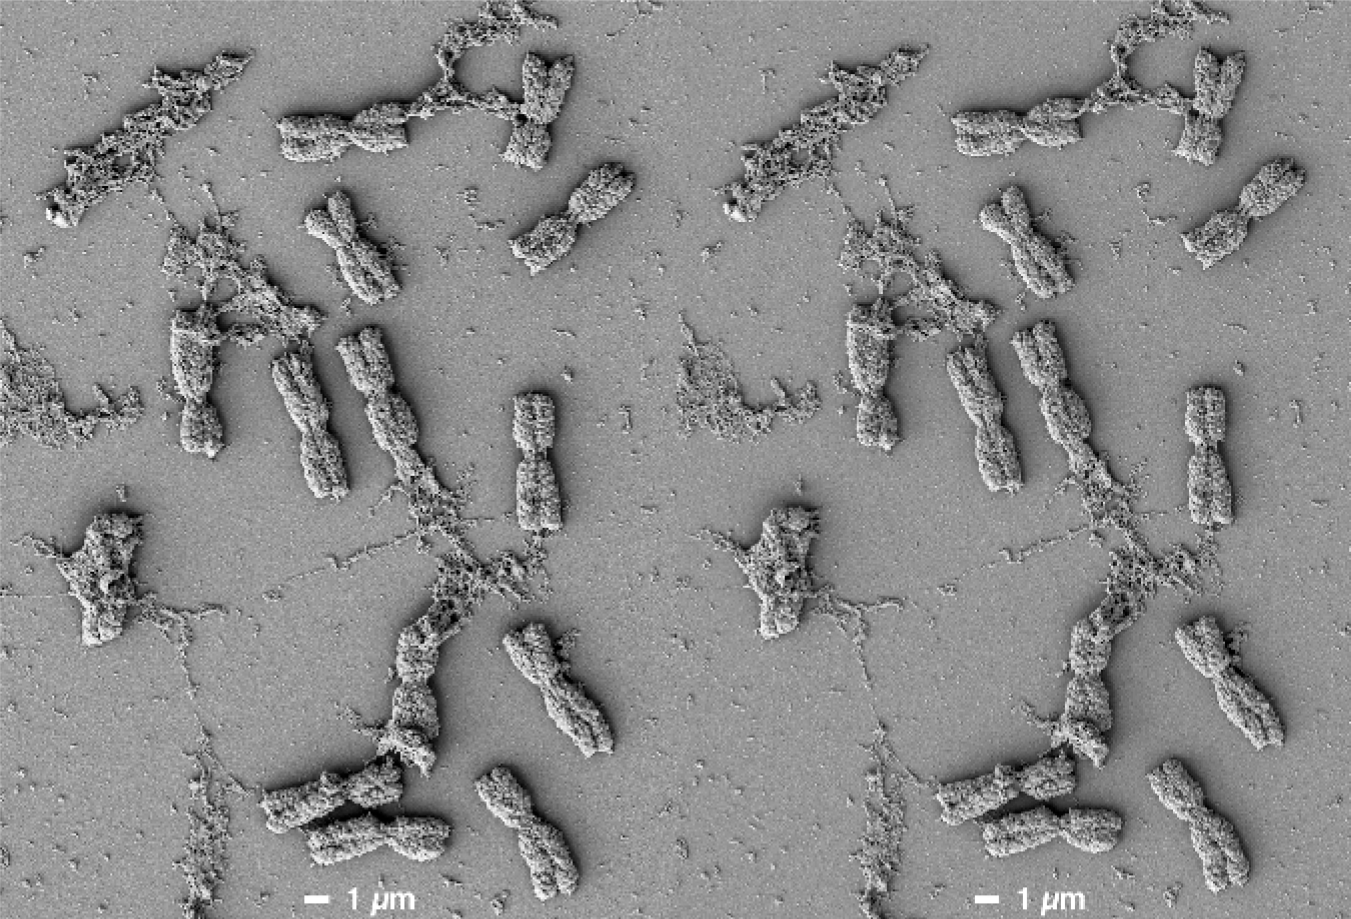
\includegraphics[keepaspectratio, width  =\textwidth]{img/barleyChroms}
			\end{column}
		\end{columns}
		
		\blfootnote{Figure from Punnett 1911}
		
	\end{frame}
	
	
	\begin{frame}
		\frametitle{What is Sequencing?}


\begin{columns}

\begin{column}{0.5\textwidth}

\centering		A genome is the complete DNA present in an individual cell or organism\\
\vspace{10pt}

DNA sequencing is the process of decoding the sequence of As, Ts, Cs and Gs in a sample of DNA 
\vspace{10pt}
\end{column}	
	\begin{column}{0.5\textwidth}
		\centering \textbf{Structure of DNA}
		
		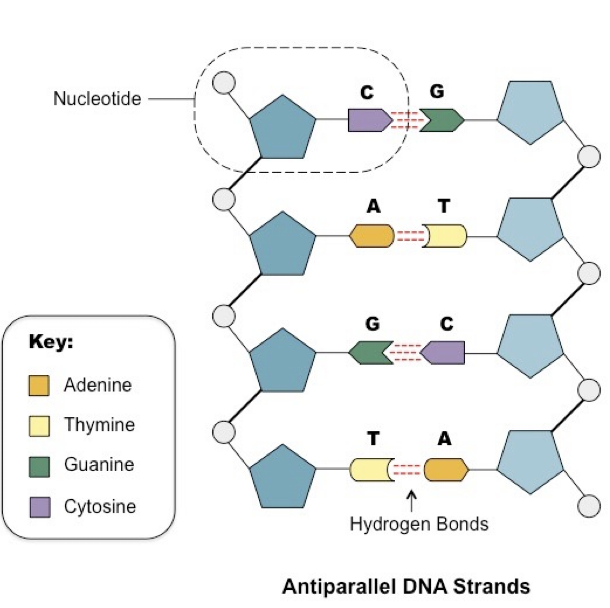
\includegraphics[keepaspectratio, width  =0.8\textwidth]{img/DNA_cartoon}
	\end{column}	
\end{columns}		\pause
	\textbf{How we measure DNA sequence data}
\centering
\small		
\begin{tabular}{|c|c|c|}
	\hline
	\textbf{Base Pairs} & \textbf{Unit} & \textbf{Example} \\
	\hline
	1 & 1bp & Single Nucleotide \\
	\hline
	1,000 & 1kbp & The average human gene is 10-15kbp long\\
	\hline
	1,000,000 & 1Mbp & The human X-chromosome is 154Mbp long \\
	\hline
	1,000,000,000 & 1Gbp & The human is genome 3.05Gbp long \\
	\hline
\end{tabular}
\end{frame}



\begin{frame}
	\centering
	
	\Huge What are some uses for genomics in forestry?
\end{frame}


\begin{frame}
	\begin{columns}
		\begin{column}{0.1\textwidth}
			
\includegraphics[keepaspectratio, width  =\textwidth]{img/dnaCartoon}
		\end{column}
		\begin{column}{0.95\textwidth}
			\frametitle{Some Uses for Genomics in UBC Forestry}
			\begin{itemize}
				\item[] Developing breeding programs
				\begin{itemize}
					\item[--] Identification of important/useful genetic variation  (e.g. targets for transformation)
					\item[--] Genome guided selection (e.g. breeding trees with specific attributes)
				\end{itemize}
				\item[ ]Identifying populations that are:
				\begin{itemize}
					\item[--] Sensitive to climate change (e.g. given climate change projections) 
					\item[--] Particularly distinct (e.g. culturally or otherwise important to stakeholders) 
				\end{itemize}
			\end{itemize}
		\end{column}
	\end{columns}
\end{frame}




\begin{frame}
	\frametitle{An Example Genomics Project}
	\centering	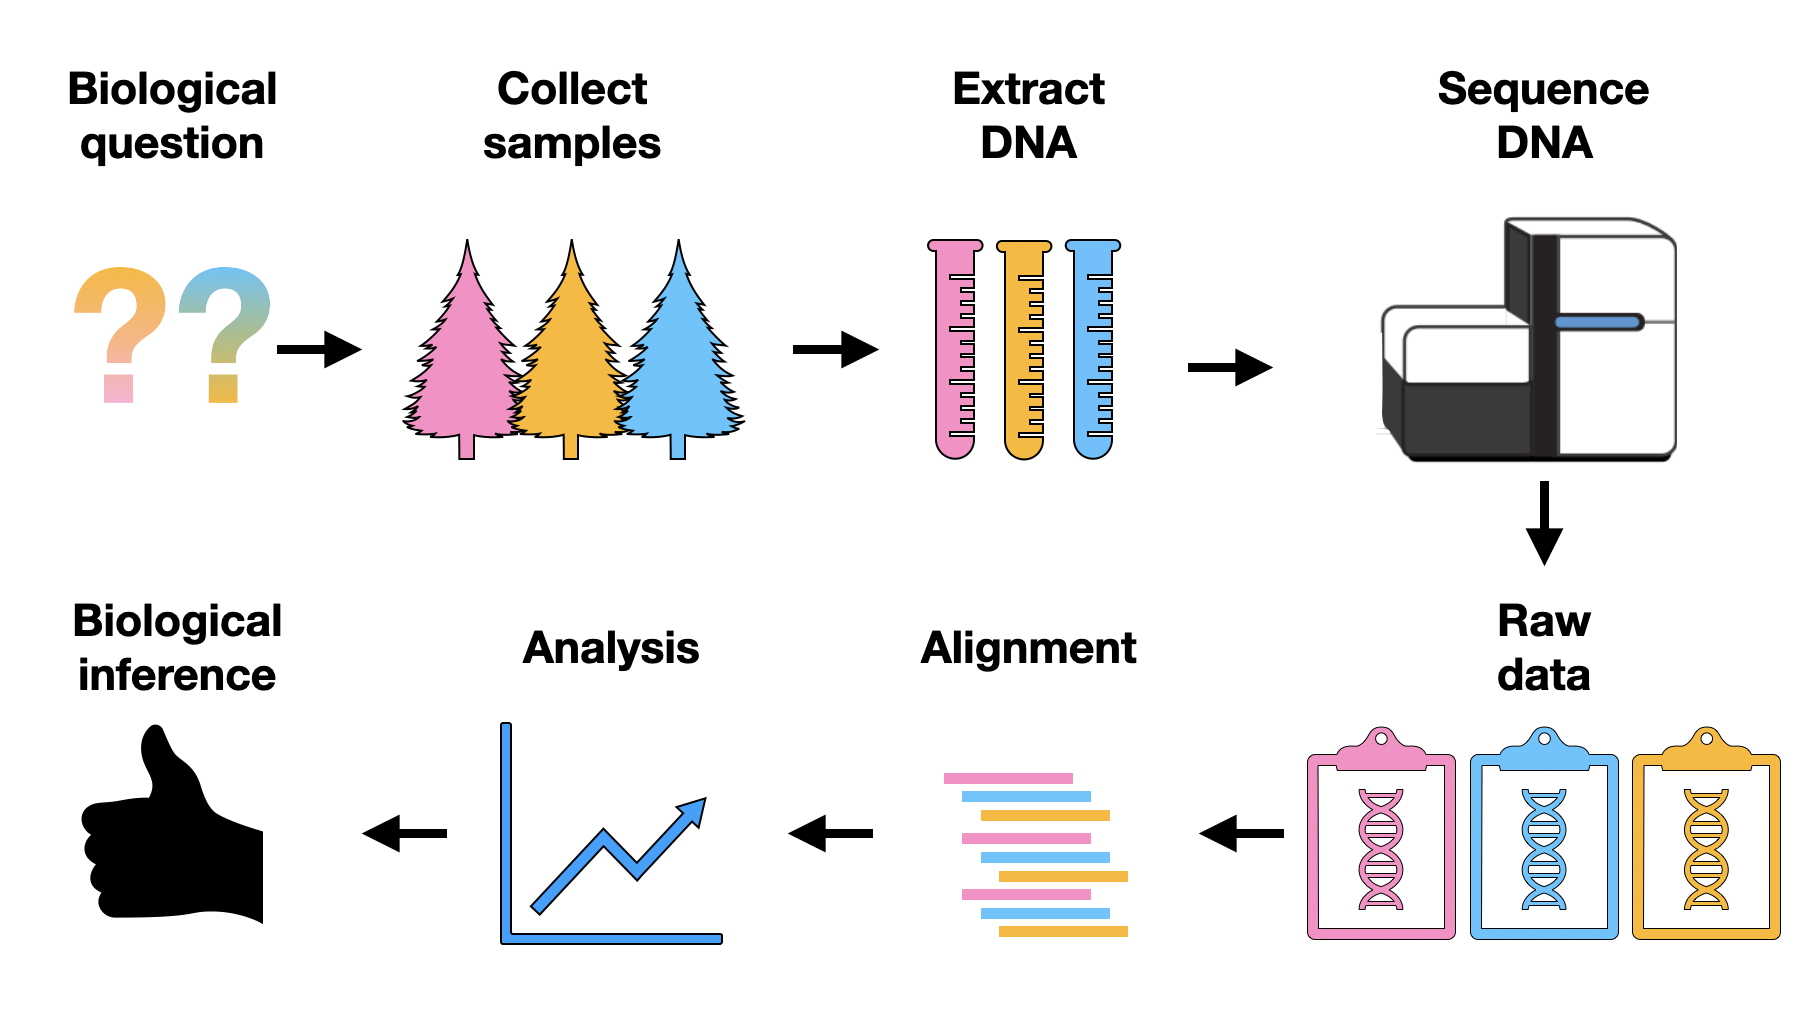
\includegraphics[keepaspectratio, width  =\textwidth]{img/bio_project}
\end{frame}

\begin{frame}
	\frametitle{An Example Genomics Project}
	\centering	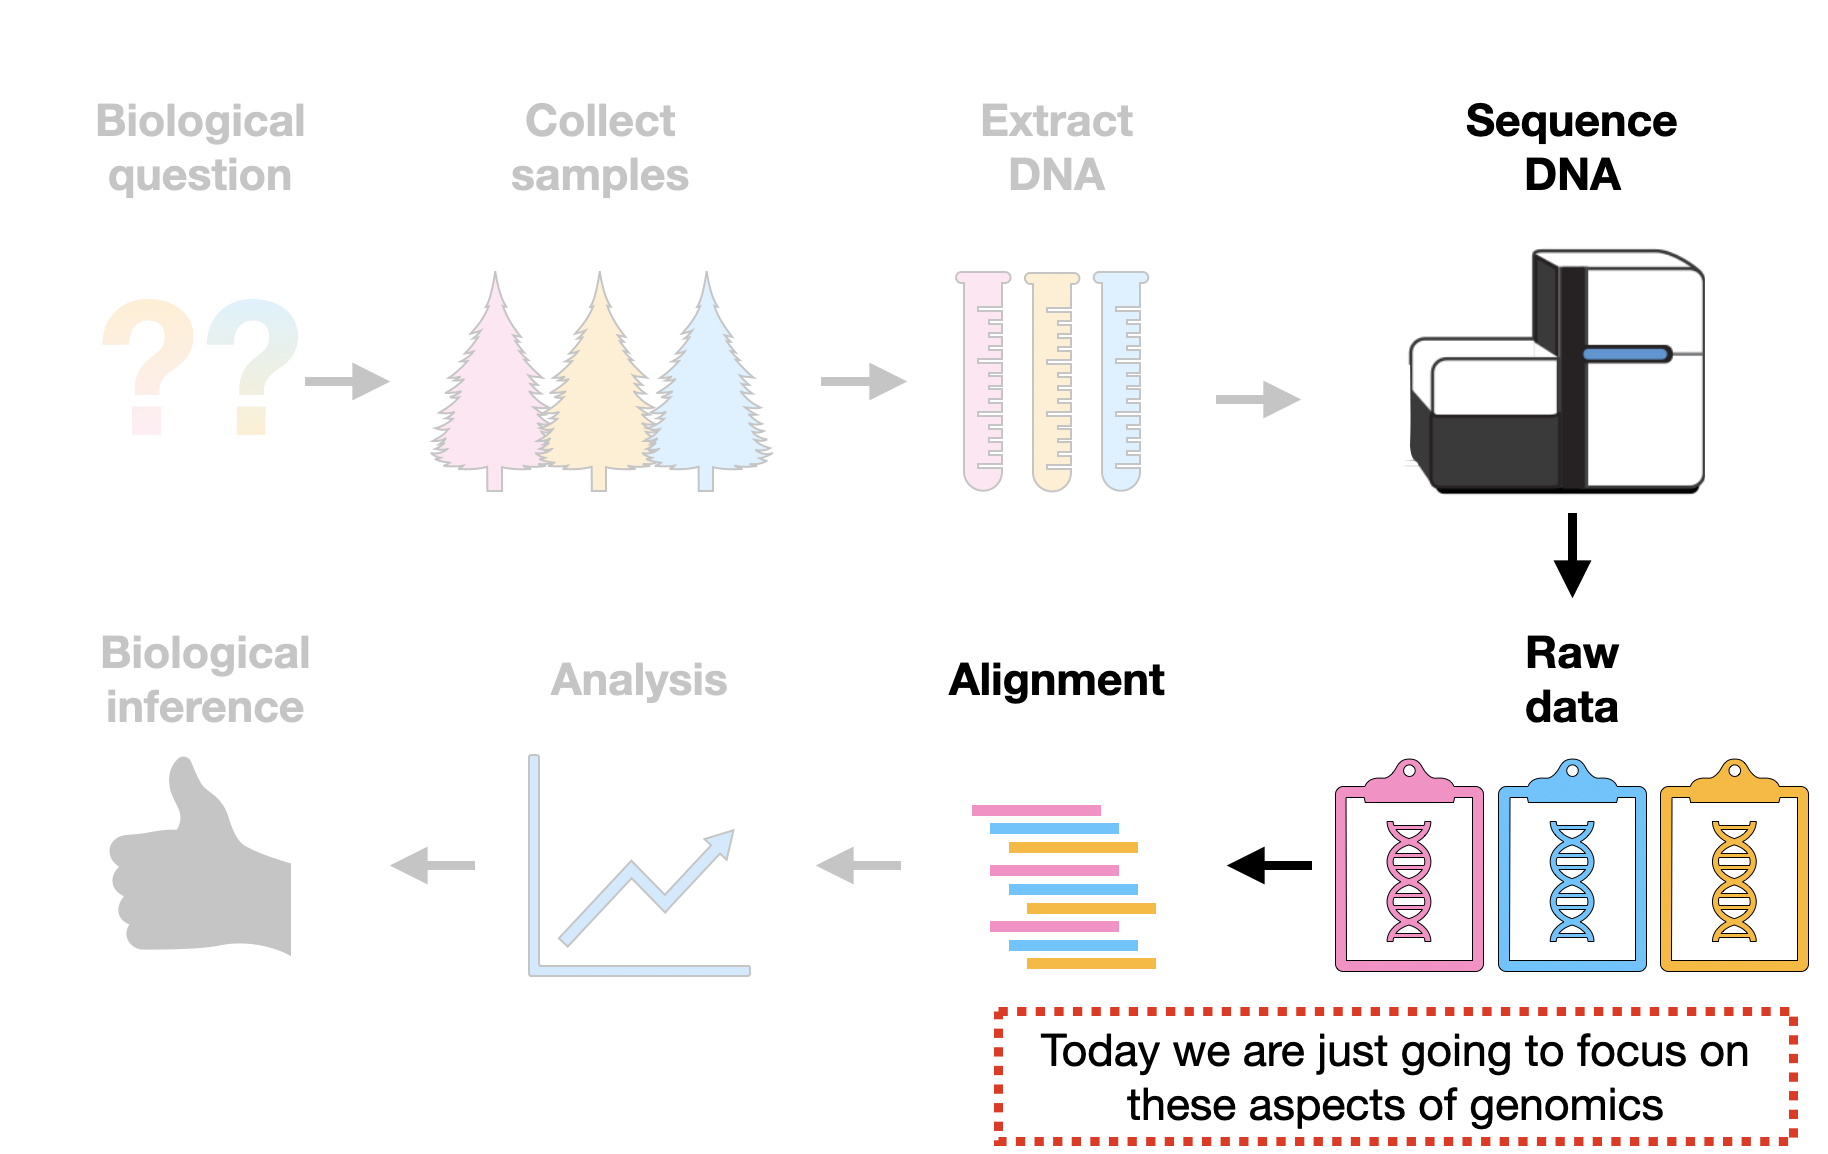
\includegraphics[keepaspectratio, width  =\textwidth]{img/bio_project_masked}
\end{frame}



\begin{frame}
	\frametitle{A Timeline of Some Discoveries}
	
	\begin{columns}
		\begin{column}{0.4\textwidth}
			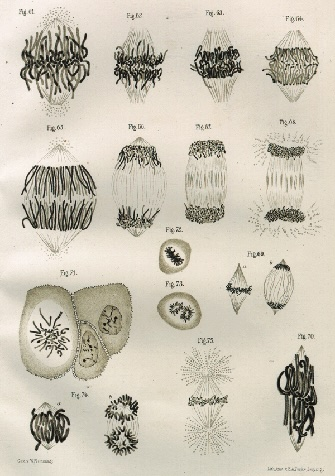
\includegraphics[keepaspectratio, width  =\textwidth]{img/chromosomes}
		\end{column}
		\begin{column}{0.6\textwidth}
			\begin{itemize}
				\small
				\item[1915] Morgan and Sturtevant constructed their genetic map for \textit{D. melanogaster}
				\item[1932] Barbara McClintock confirms that genes are exchanged during crossing-over
				\item[1940s] DNA is determined to be the material within chromosomes that carry heritable information
				\item[1950] The composition of DNA is determined - including Chargaff's rules
				\item[1953] The structure of DNA is determined
				
				
			\end{itemize}
		\end{column}
		
	\end{columns}
	\blfootnote{Drawing of mitosis by Walther Flemming 1882}
	
	
\end{frame}	

\begin{frame}
	\frametitle{DNA Replication}
	\begin{columns}
		\begin{column}{0.6\textwidth}
			\begin{itemize}
				\item[--] Both mitosis and meiosis involve DNA replication
				\item[--] DNA replication produces two identical replicas of DNA from one original DNA molecule. 
				\item[--] During replication, the double-stranded DNAs are separated. Each strand of the original DNA molecule serves as a template for the production of its counterpart.
				\item[--]This process occurs in all living organisms and is the basis for growth and inheritance. 	
				\blfootnote{Image from: \textit{Wikipedia}}
			\end{itemize}		
		\end{column}			
		\begin{column}{0.5\textwidth}
			\centering 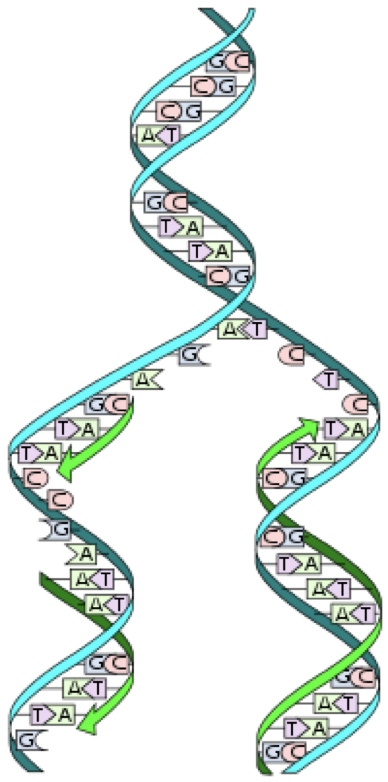
\includegraphics[keepaspectratio, width  =0.75\textwidth]{img/DNA_replication} 
		\end{column}
	\end{columns}
\end{frame}


\begin{frame}
	\frametitle{The Polymerase Chain Reaction - PCR}
\centering	PCR is a technique to amplify a single copy or a few copies of a piece of DNA to millions of copies of a particular DNA sequence. 
			\centering 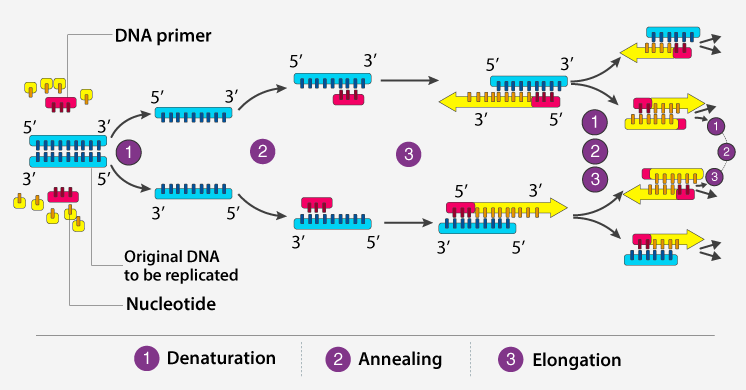
\includegraphics[keepaspectratio, width  =\textwidth]{img/PCR} 
			\blfootnote{Image modifed from: \url{https://byjus.com/biology/pcr/}}
\end{frame}

\begin{frame}
	\frametitle{Applications of PCR}
	
	\begin{columns}
\begin{column}{0.5\textwidth}
Developed in the early 1980s, PCR is fundamental in modern biology and is widely used in clinical and research settings for:
			\begin{itemize}
\item[--] DNA cloning for sequencing
\item[--] Functional analysis of genes 
\item[--] Diagnosis of hereditary diseases
\item[--] DNA fingerprinting
\item[--] Detection and diagnosis of infectious diseases. 
\end{itemize}
In 1993, Mullis and Michael Smith (UBC) was awarded the Nobel Prize in Chemistry
		\end{column}			
\begin{column}{0.5\textwidth}
\centering 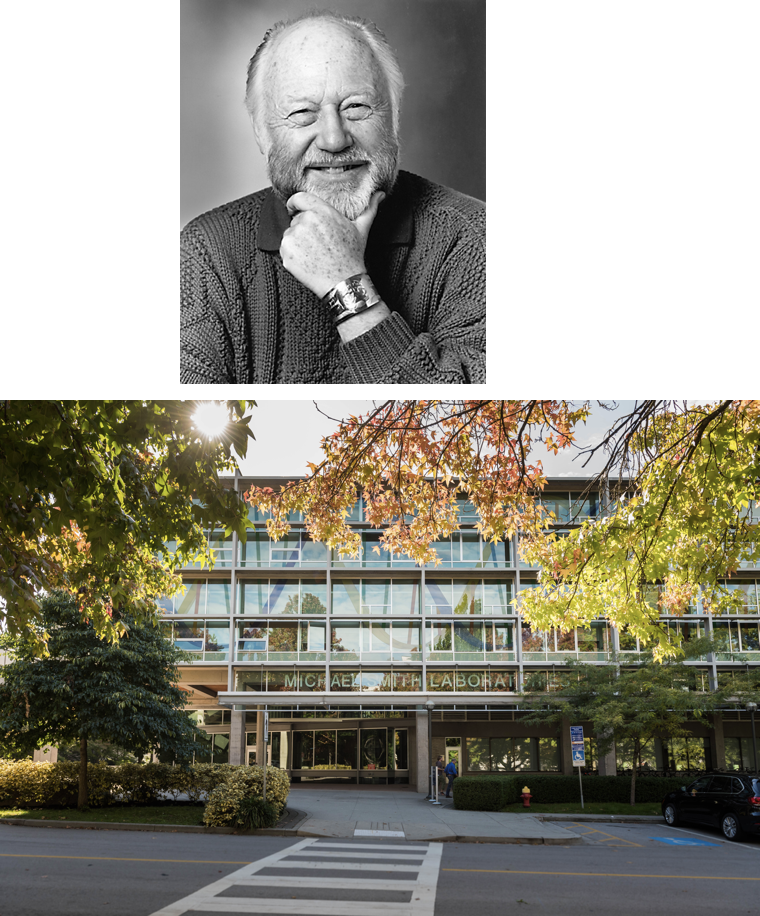
\includegraphics[keepaspectratio, width  =\textwidth]{img/PCR_MichaelSmith} 
\end{column}
\end{columns}


\end{frame}



\begin{frame}
	
	\frametitle{Technological Milestones}
	
	\begin{columns}
		\begin{column}{0.1\textwidth}
			
\includegraphics[keepaspectratio, width  =\textwidth]{img/dnaCartoon}
		\end{column}
		\begin{column}{0.9\textwidth}
			\scriptsize 
			\begin{itemize}
				\item[1953] \textbf{\underline{Sequencing of insulin protein}}
				\item[1965] Sequencing of alanine tRNA
				\item[1977] Maxam–Gilbert sequencing
				\item[1977] \textbf{\underline{Sanger sequencing}}
				\item[1990] Paired-end sequencing
				\item[2000] Massively parallel signature sequencing by ligation
				\item[2003] \textbf{\underline{Single-molecule massively parallel sequencing-by-synthesis}}
				\item[2003] Sequencing by synthesis of in vitro DNA colonies in gels
				\item[2007] Large-scale targeted sequence capture
				\item[2010] Direct detection of DNA methylation during single-molecule sequencing
				\item[2010] Single-base resolution electron tunnelling through a solid state detector
				\item[2011] Semiconductor sequencing by proton detection
				\item[2012] \underline{\textbf{Reduction to practice of nanopore sequencing}}
				\item[2012] Single-stranded library preparation method for ancient DNA
				
			\end{itemize}
		\end{column}
	\end{columns}
\end{frame}



\begin{frame}

\frametitle{DNA Sequencing - Sanger}


			\centering 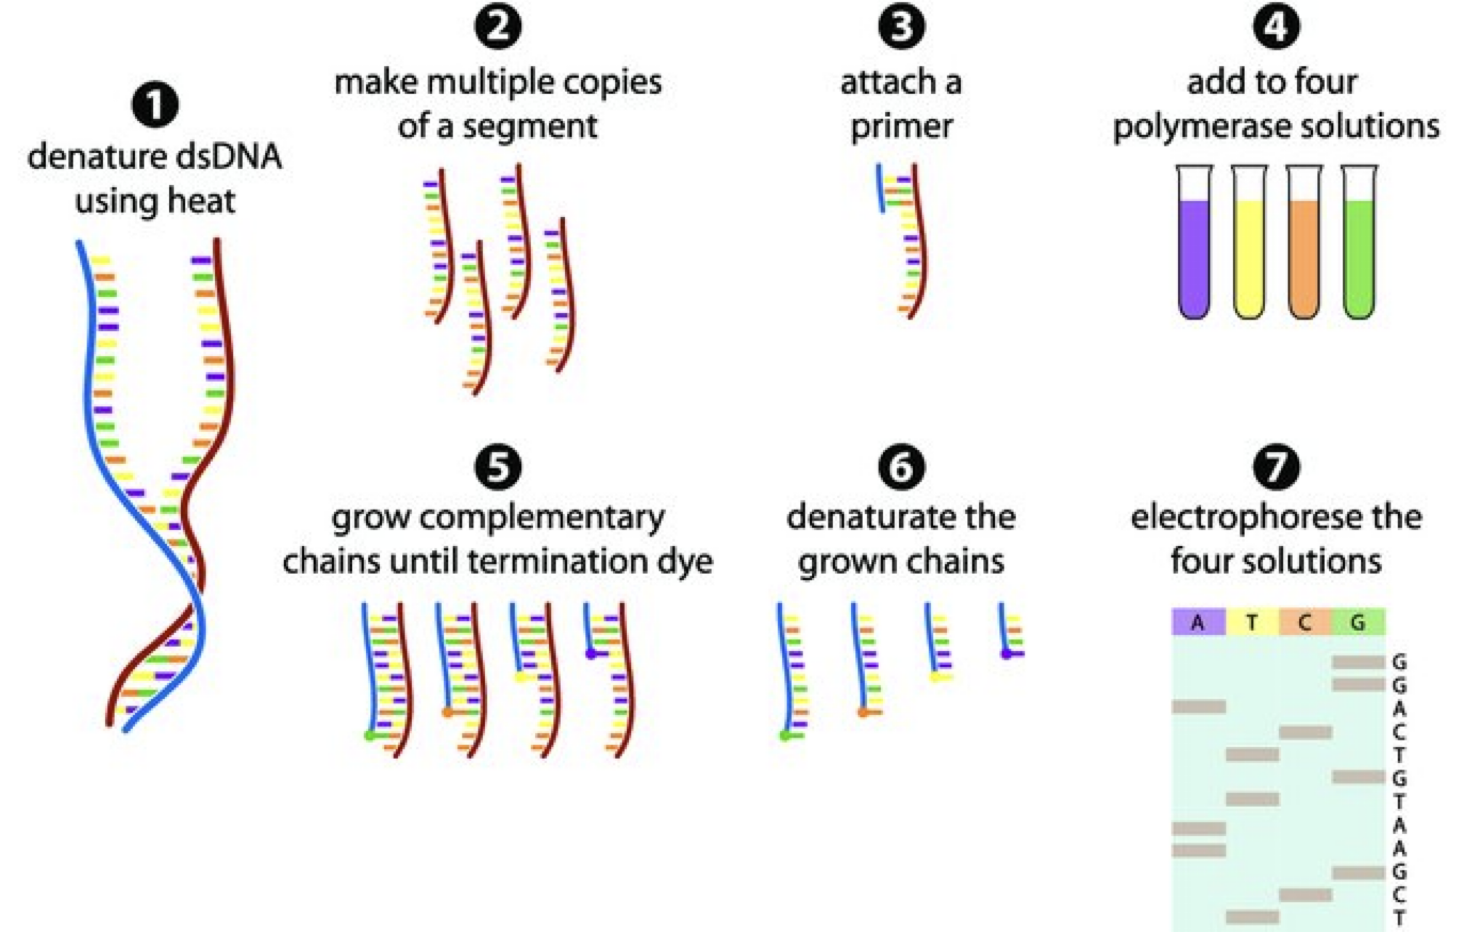
\includegraphics[keepaspectratio, width  =\textwidth]{img/sangerSequencing} 
			
			
\blfootnote{Developed by Frederick Sanger and colleagues in the 1970s
\\ Figure from PhD thesis of Michel G. Gauthier}
\end{frame}


\begin{frame}
	
	\frametitle{DNA Sequencing - Sanger}
	
	
	\centering 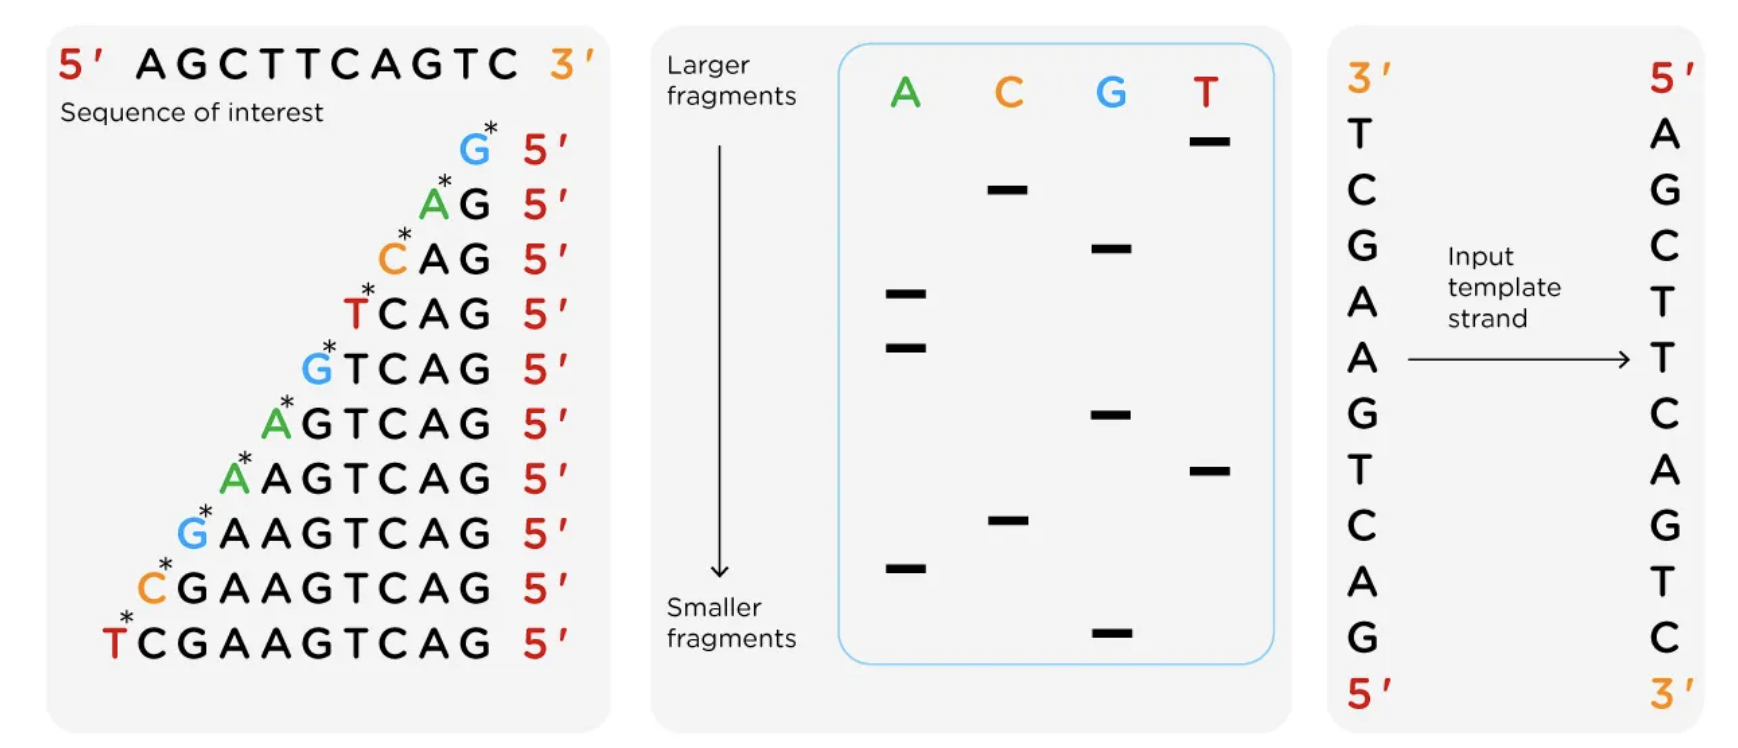
\includegraphics[keepaspectratio, width  =\textwidth]{img/sanger} 
	
	\textit{The sequence identified from the gel will be the reverse complement of the input sequence!}
	
	\blfootnote{\url{https://jackwestin.com/resources/mcat-content/recombinant-dna-and-biotechnology/dna-sequencing}}
	



\end{frame}



\begin{frame}
	
	\frametitle{DNA Sequencing - Sanger}
	\small
	\begin{columns}
		\begin{column}{0.5\textwidth}
			\begin{itemize}
				\item[--] Gold standard for accuracy (99.99\% accurate)
			    \item[--] Cheap equipment (low initial investment)
				\item[--] Labour intensive
				\item[--] Can only be used for short DNA strands (100 to 1000 base pairs)
				\item[--] Time consuming \& low throughput
				\item[--] The basis of the human genome project
			\end{itemize}
		\end{column}
		\begin{column}{0.34\textwidth}	
				\centering 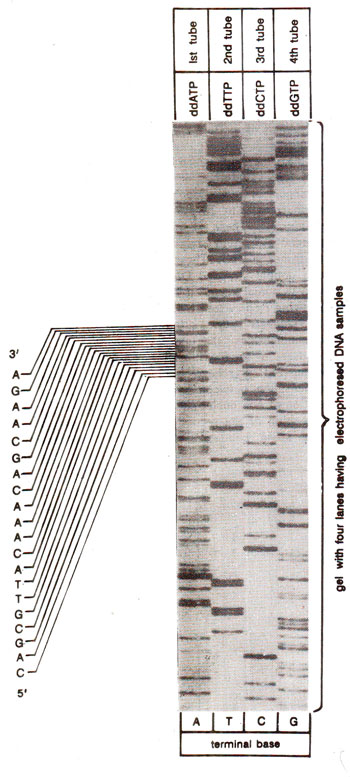
\includegraphics[keepaspectratio, width  =\textwidth]{img/sangerGel} 
			\end{column}
			\end{columns}		
			
\end{frame}


\begin{frame}
	
	\frametitle{Genome Milestones}
	
	\begin{columns}
		\begin{column}{0.1\textwidth}
			
\includegraphics[keepaspectratio, width  =\textwidth]{img/dnaCartoon}
		\end{column}
		\begin{column}{0.9\textwidth}

			\begin{itemize}
\item[1977] Bacteriophage $\phi$X174
\item[1982] Bacteriophage $\lambda$
\item[1995] \textit{Haemophilus influenzae}
\item[1996] \textit{Saccharomyces cerevisiae}
\item[1998] \textit{Caenorhabditis elegans}
\item[2000] \textit{Drosophila melanogaster}
\item[2000] \textit{Arabidopsis thaliana} -\small{ The first plant genome sequenced! } \normalsize
\item[2001] \textit{Homo sapiens}
\item[2002] \textit{Mus musculus}
\item[2004] \textit{Rattus norvegicus}
\item[2005] \textit{Pan troglodytes}
\item[2005] \textit{Oryza sativa}
				
			\end{itemize}
		\end{column}
	\end{columns}
\end{frame}



\begin{frame}
	\frametitle{Genome Sequencing}
	Genome sequencing is now a routine part of genetic research\\
	\vspace{10pt}
	\centering 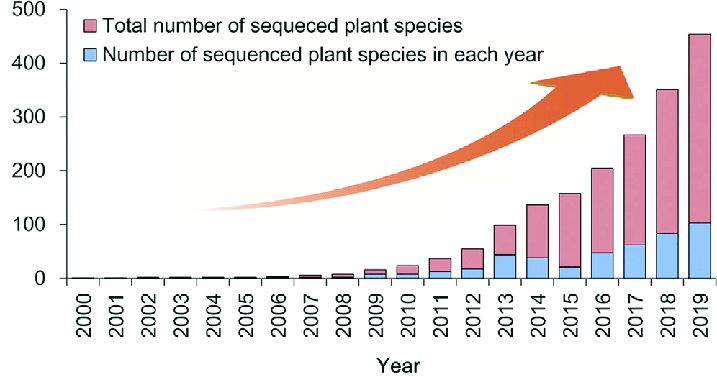
\includegraphics[keepaspectratio, width  =\textwidth]{img/plantGenomes} 
	\blfootnote{From: Tang et al. 2019 \textit{Plant Communications}}
\end{frame}


\begin{frame}
	\frametitle{DNA Sequencing - Costs}

	\centering 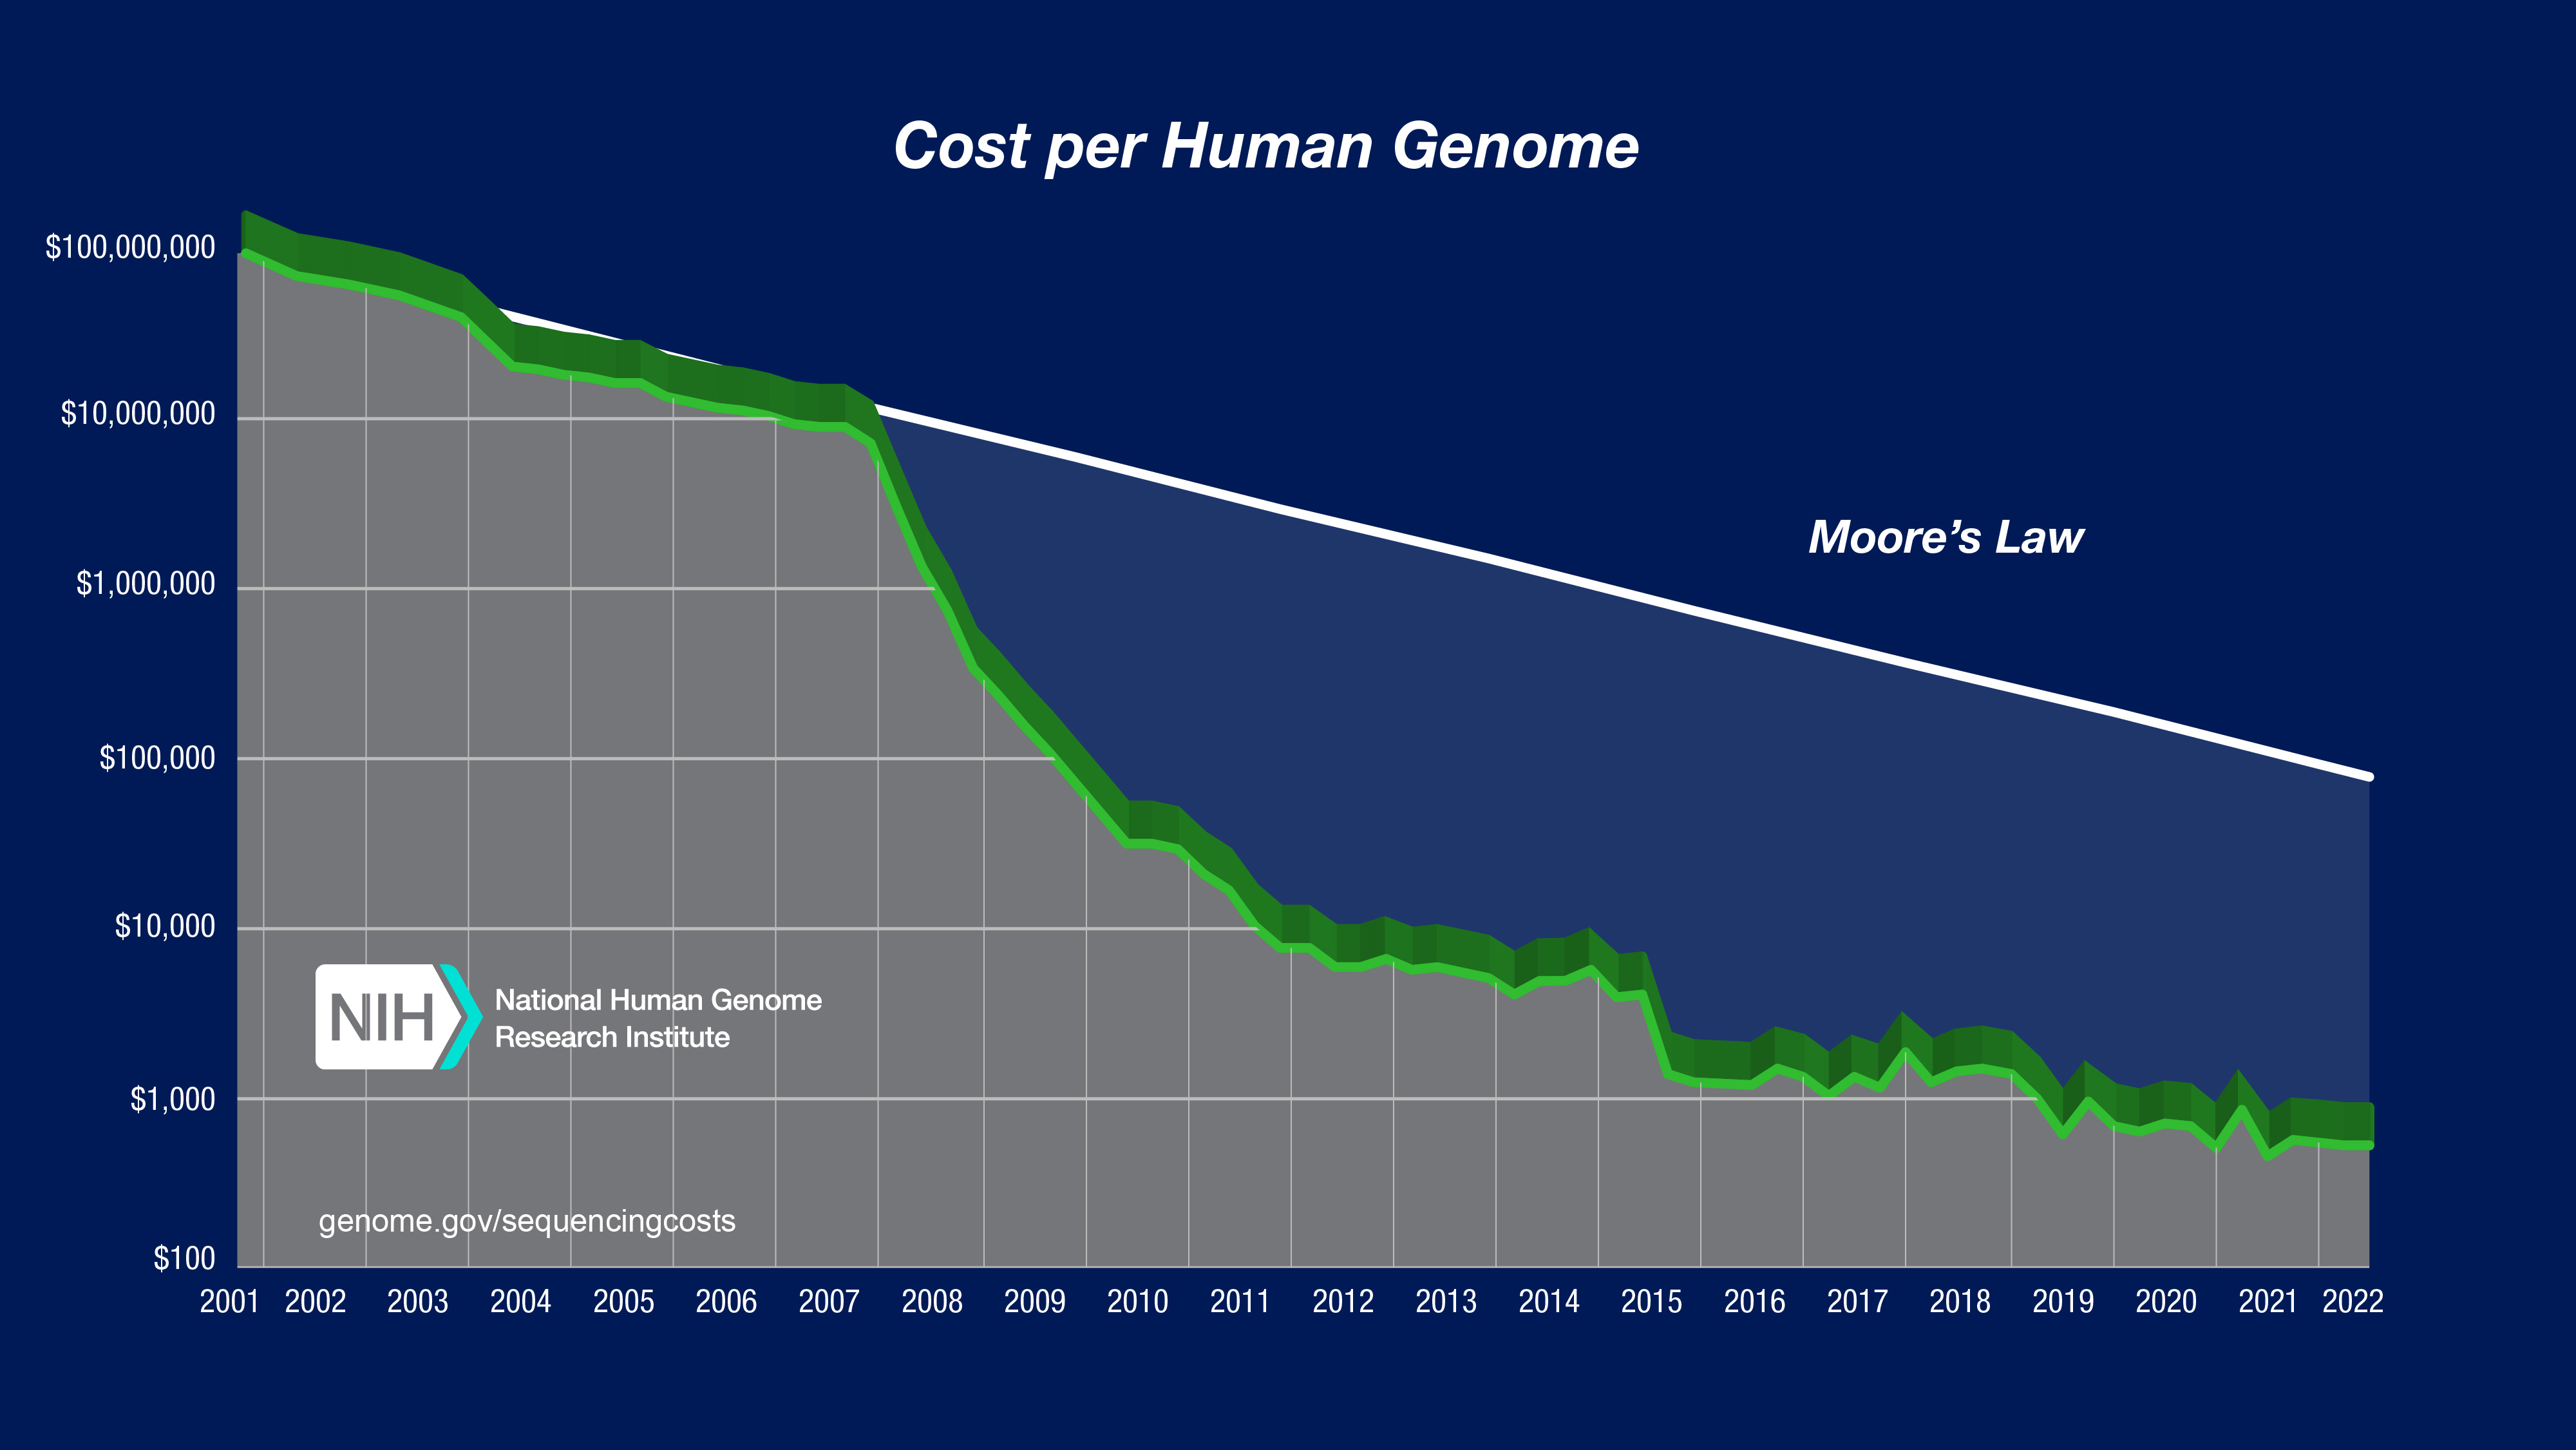
\includegraphics[keepaspectratio, width  =\textwidth]{img/mooresLaw} 
	\blfootnote{\url{https://www.genome.gov/about-genomics/fact-sheets/DNA-Sequencing-Costs-Data}}
\end{frame}


\begin{frame}
	\frametitle{DNA Sequencing}

The rapid accceleration in genome science has been facilitated by technological advances in sequencing technology

\begin{center}

$
\begin{array}{l}
	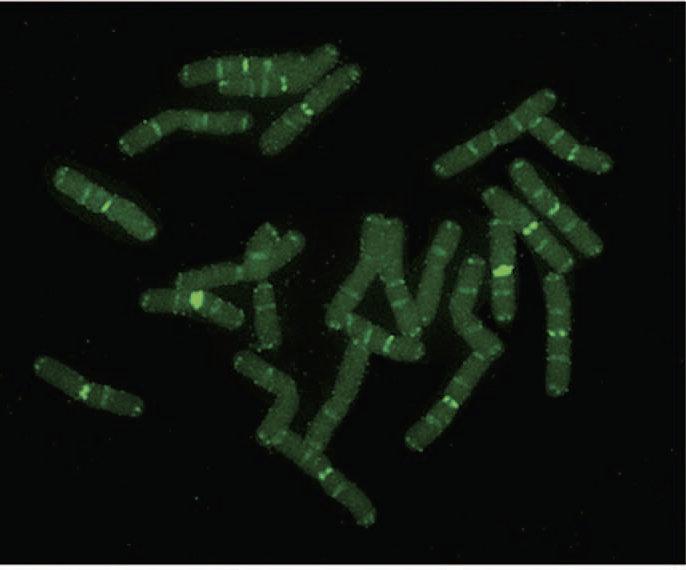
\includegraphics[width=0.3\textwidth]{img/loblollyChroms}
\end{array}
$
$\rightarrow$
$
\begin{array}{l}
	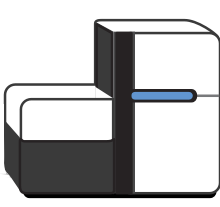
\includegraphics[width=0.3\textwidth]{img/sequencer}
\end{array}
$
\end{center}
 
\textbf{DNA sequencing machines}

\begin{itemize}
	\item[--] There are numerous technologies available
	\item[--] The various technologies have different attributes
\end{itemize}

\end{frame}


\begin{frame}
	\frametitle{DNA Sequencing - Illumina technology}
\begin{columns}
	\begin{column}{0.5\textwidth}
			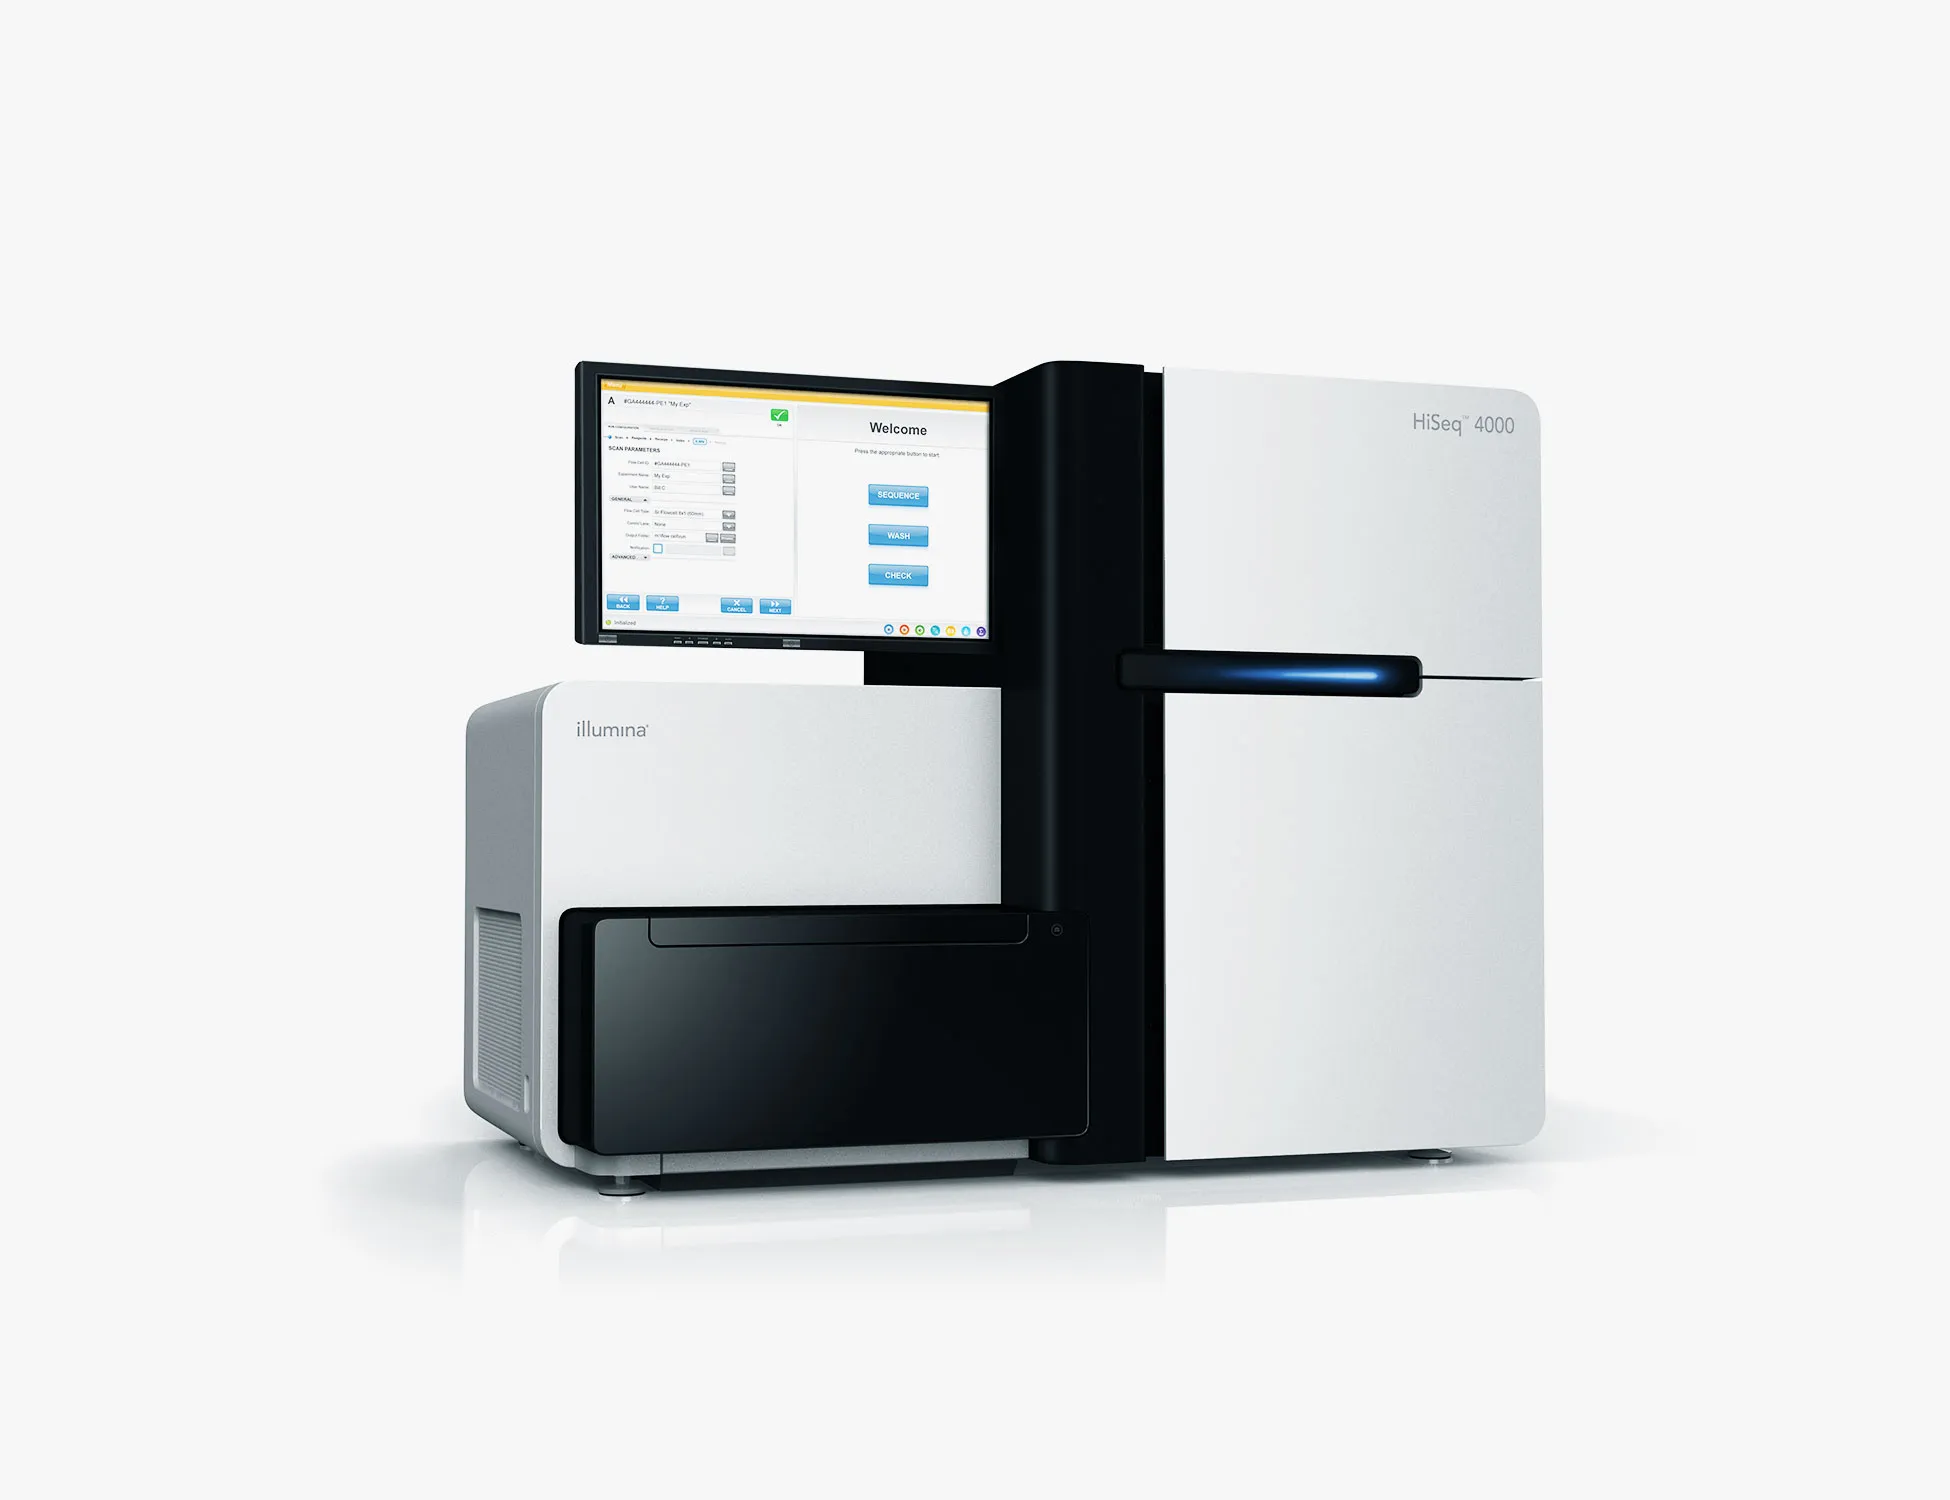
\includegraphics[width=\textwidth]{img/hiSeq}
	\end{column}
	\begin{column}{0.5\textwidth}
\begin{itemize}
\item[--] Based on sequencing by synthesis - chain elongation without termination
\item[--] Solves the problem of throughput
\item[--] Sequence millions of DNA fragments at the same time
\item[--] MASSIVE parallelization
\end{itemize}
	\end{column}
	\end{columns}
\blfootnote{There are/were several other companies in this space, but they have mostly been eclipsed by Illumina}

\end{frame}


\begin{frame}
	\frametitle{DNA Sequencing - Illumina technology}
			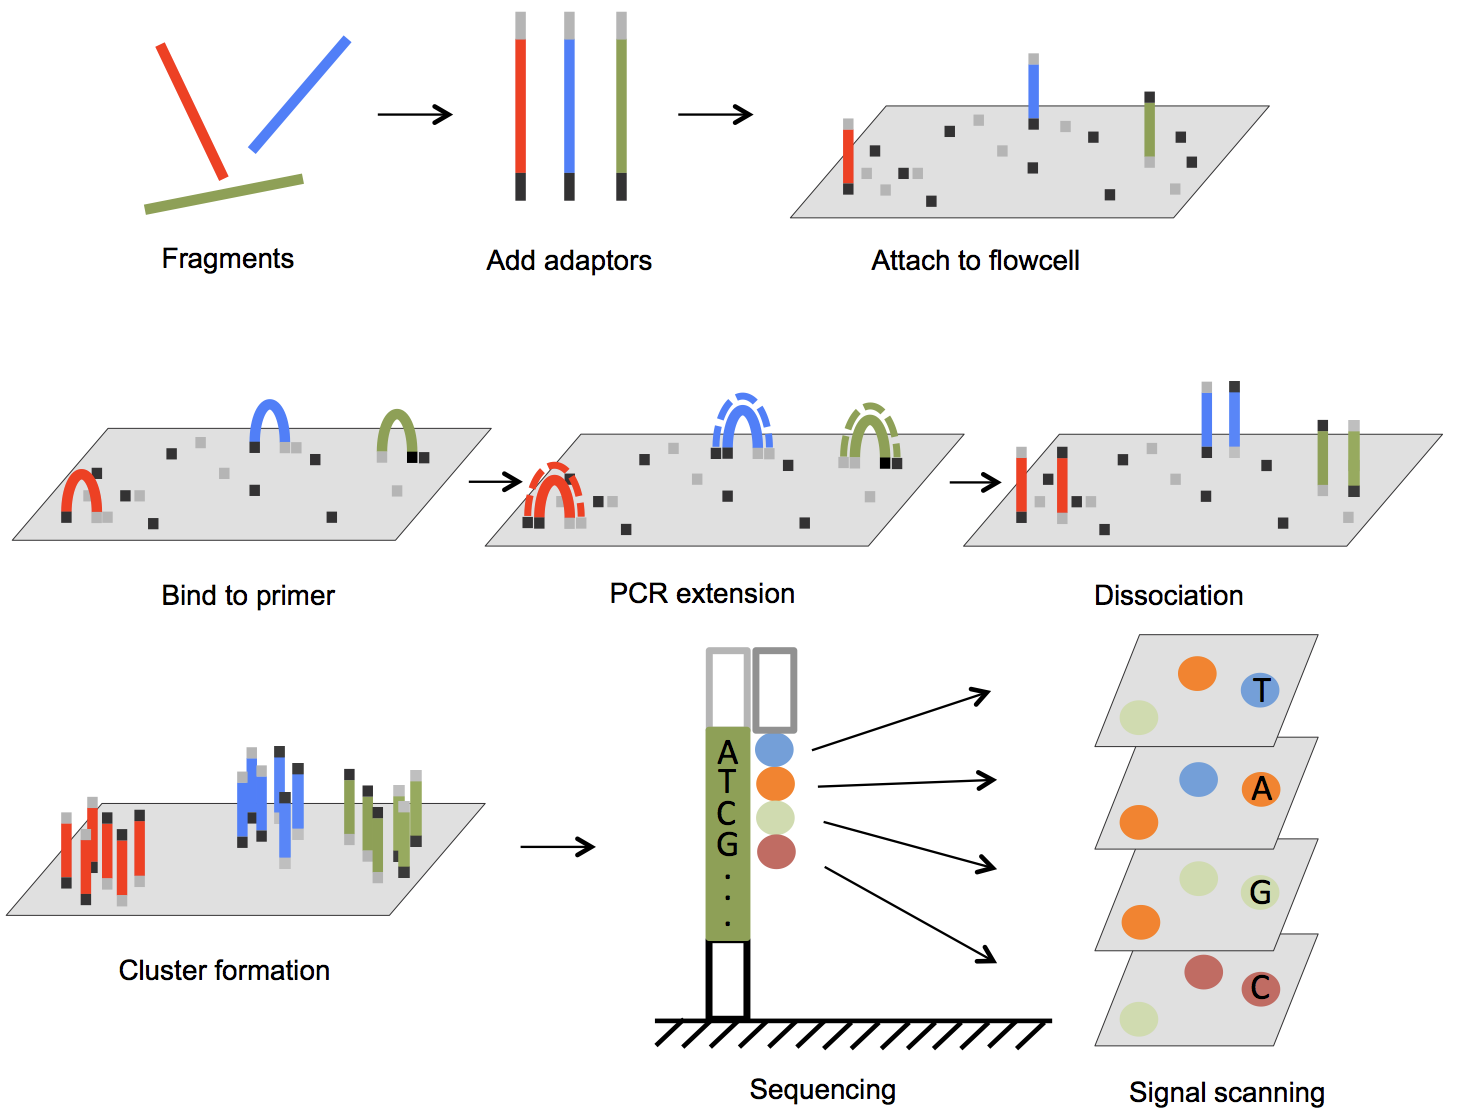
\includegraphics[width=\textwidth]{img/illumina}
\end{frame}

\begin{frame}
	\frametitle{Genome Sequencing}
		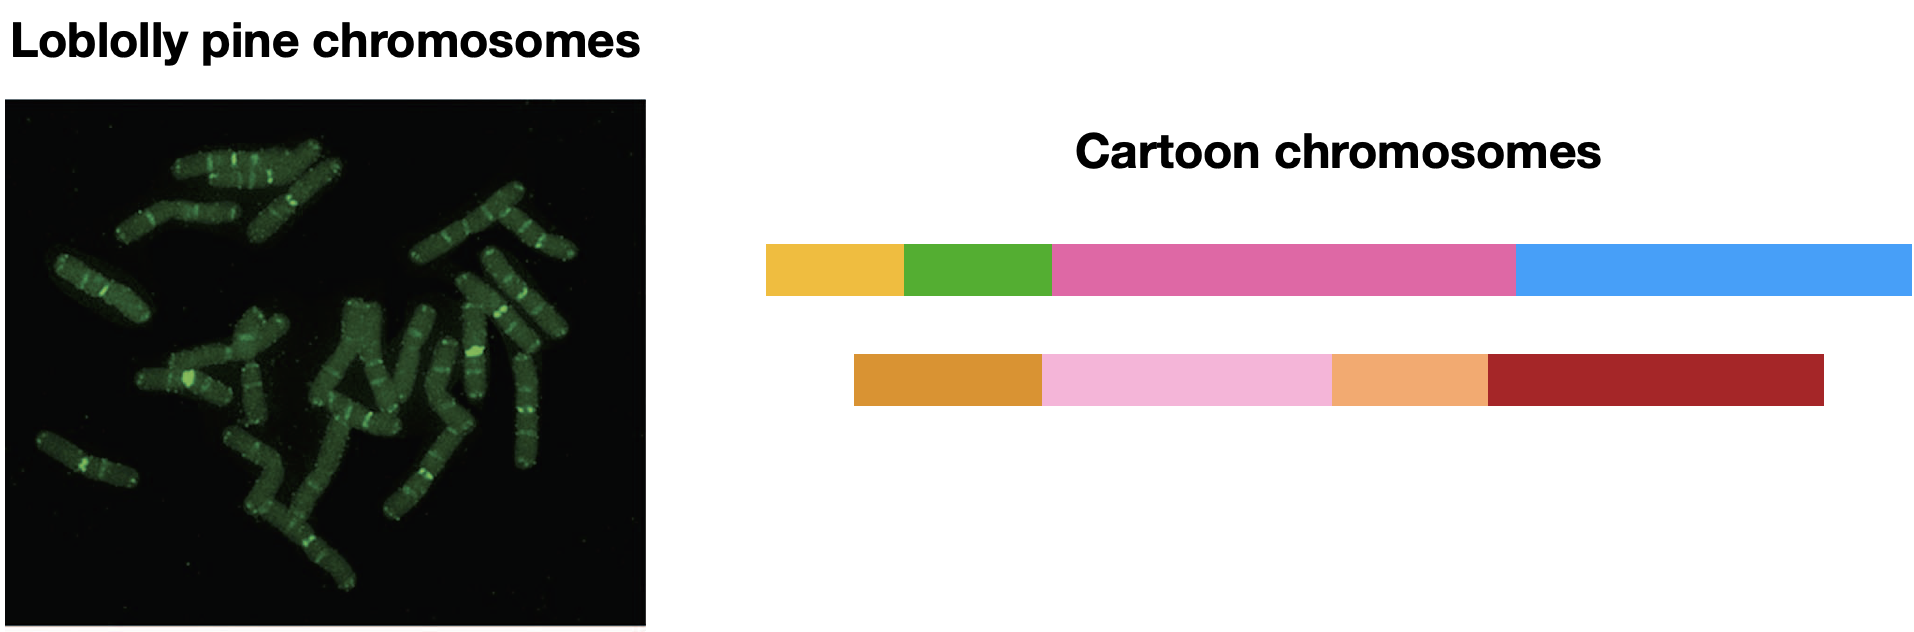
\includegraphics[width=\textwidth]{img/loblolly2cartoon}
\end{frame}


\begin{frame}
		\frametitle{Genome Sequencing}
		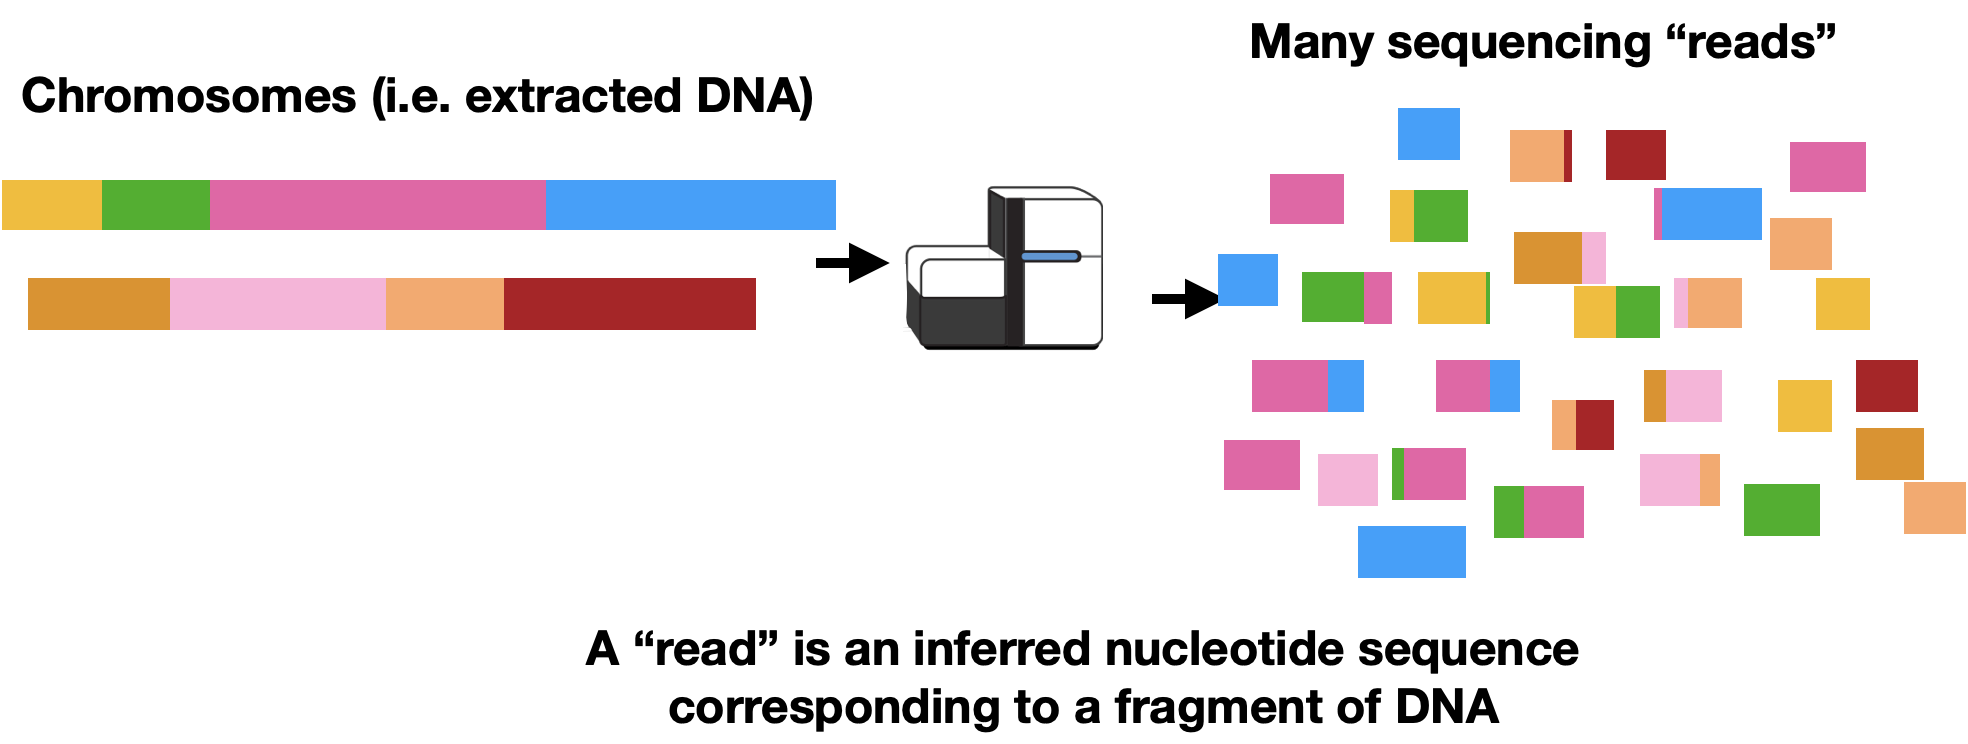
\includegraphics[width=\textwidth]{img/chroms2reads}
		\blfootnote{This basic idea has been around since the 1980s (\textit{i.e. shotgun sequencing}), but represents the foundation of how we do genome sequencing today}
\end{frame}

\begin{frame}
	\frametitle{Genome Sequencing}
	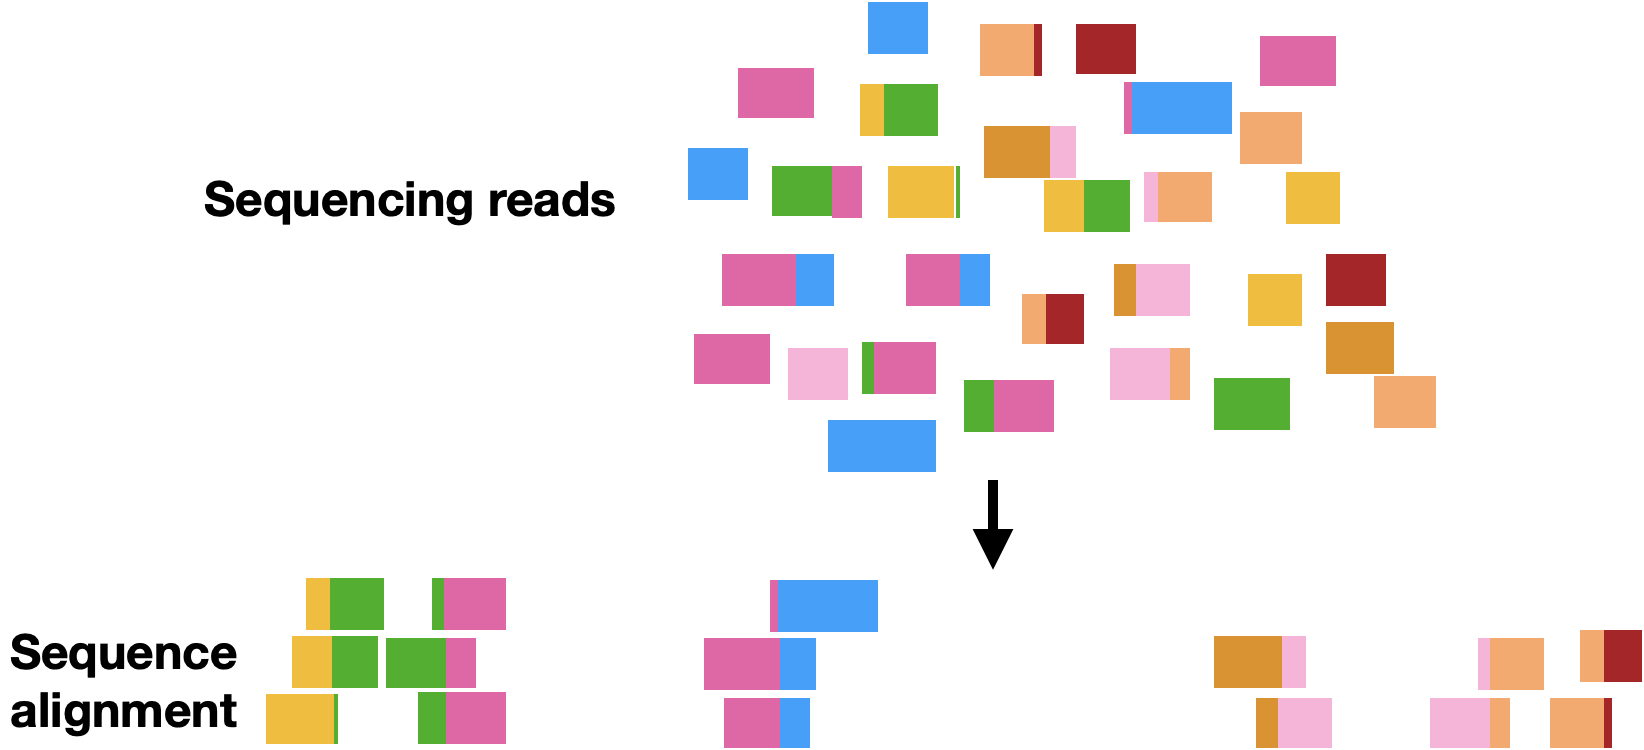
\includegraphics[width=\textwidth]{img/reads2Alignment}
	\blfootnote{This step involves identifying overlaps between reads - it can involve \textit{LOT} of computation}
\end{frame} 

\begin{frame}
	\frametitle{Genome Sequencing}
	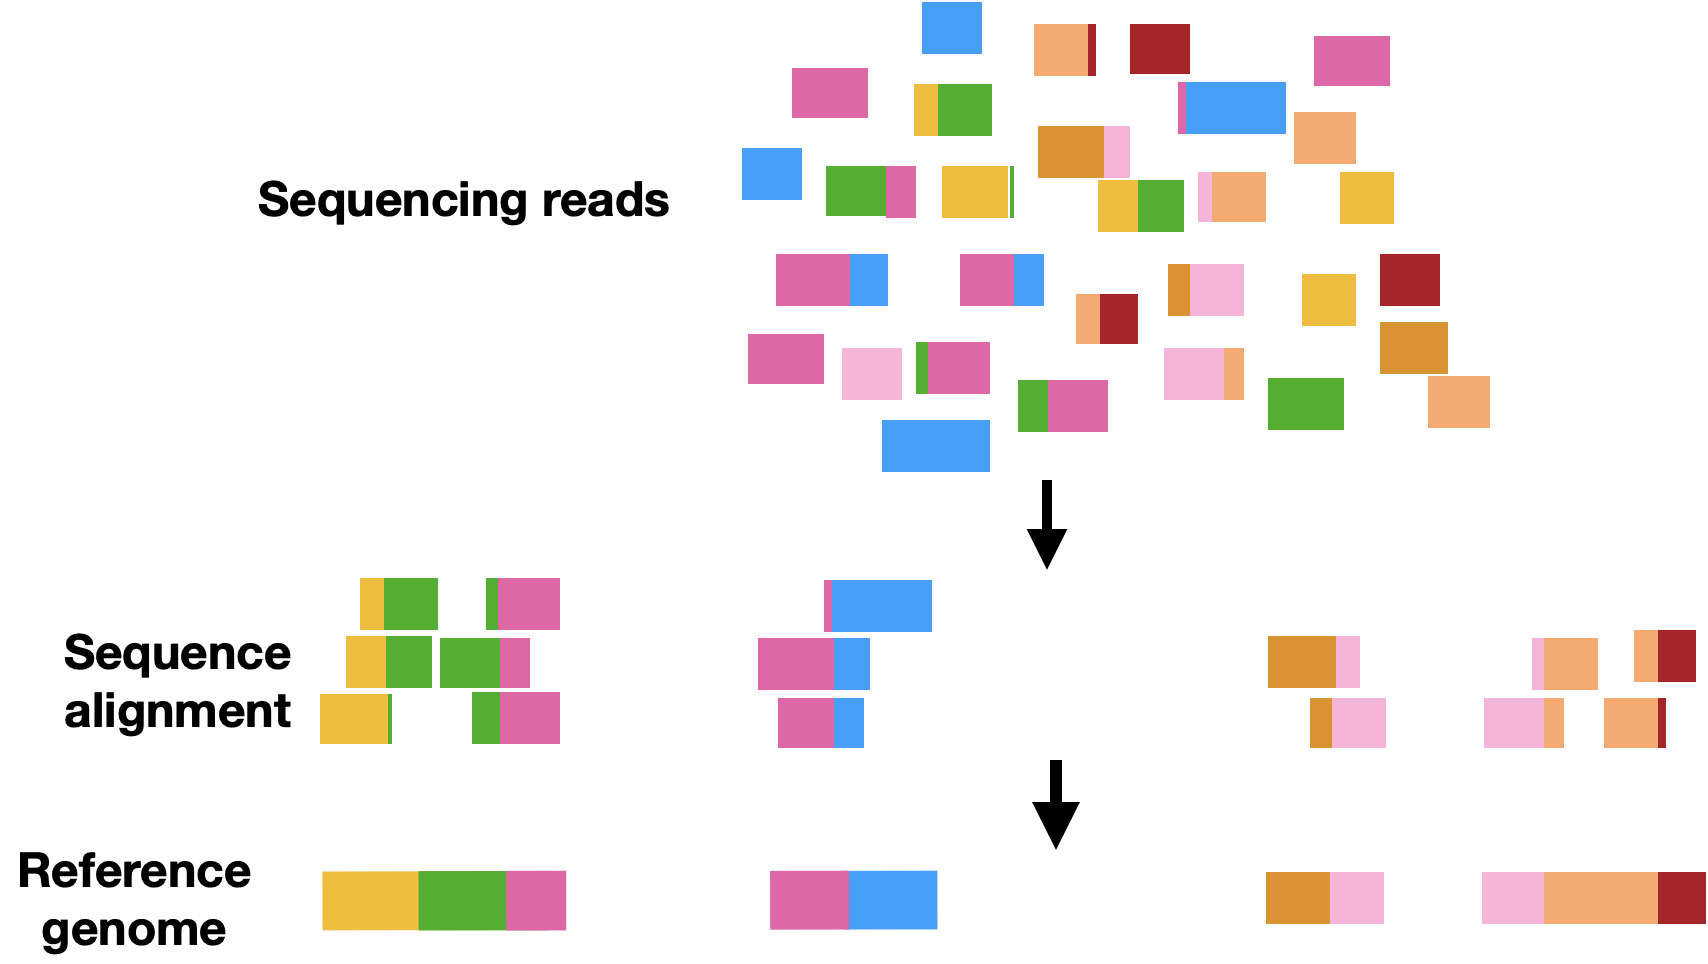
\includegraphics[width=\textwidth]{img/alignment2reference}
	\blfootnote{The alignment of the sequencing reads is used to reconstruct the input sequence }
\end{frame}

\begin{frame}
	\frametitle{Genome Sequencing - Reference Genome}

A reference genome is a representation of the average genome for a species/population
\begin{itemize}
	\item Used as the template against which to evaluate genetic variation\textsuperscript{see lecture on genetic variation}
	\item Reference genomes are incomplete pictures\\
	\vspace{20pt}
		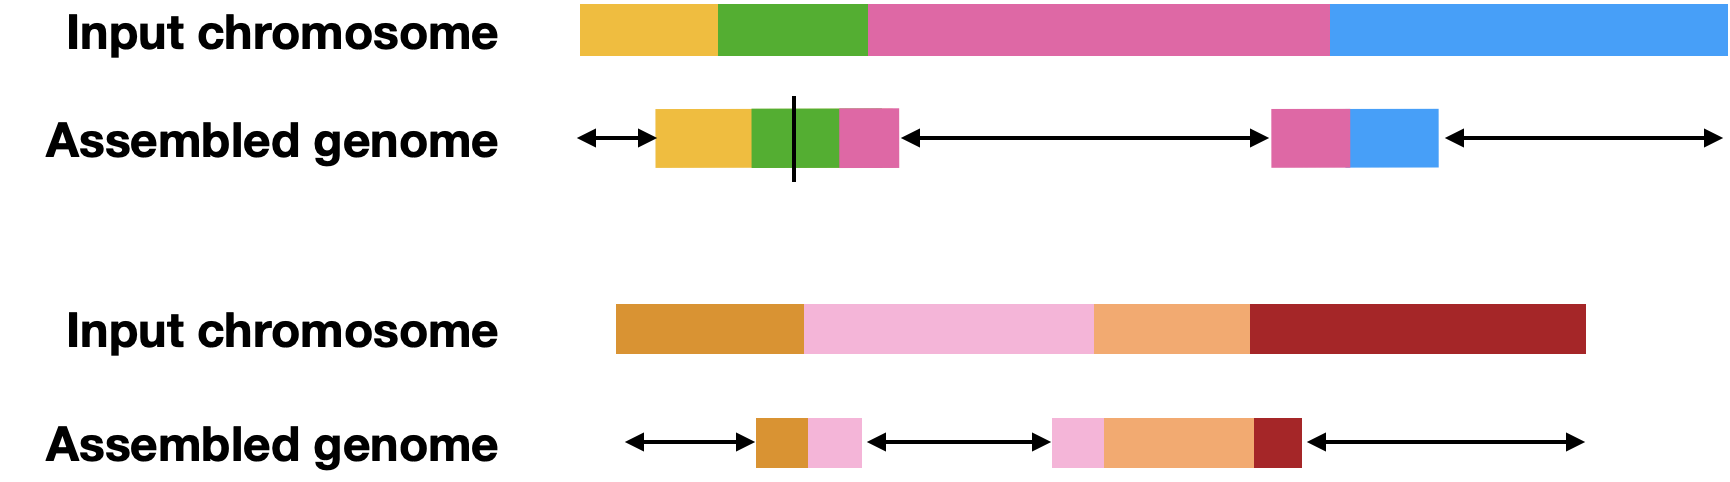
\includegraphics[width=\textwidth]{img/shortReadReference}
\end{itemize}
\end{frame}

\begin{frame}

	\Large{The Land of Waldos - Martin Handford}
\center		\includegraphics[width=0.7\textwidth]{img/Waldo}\\

	\Large Any questions? \pause Let's take a short break


\end{frame}


\begin{frame}
\center		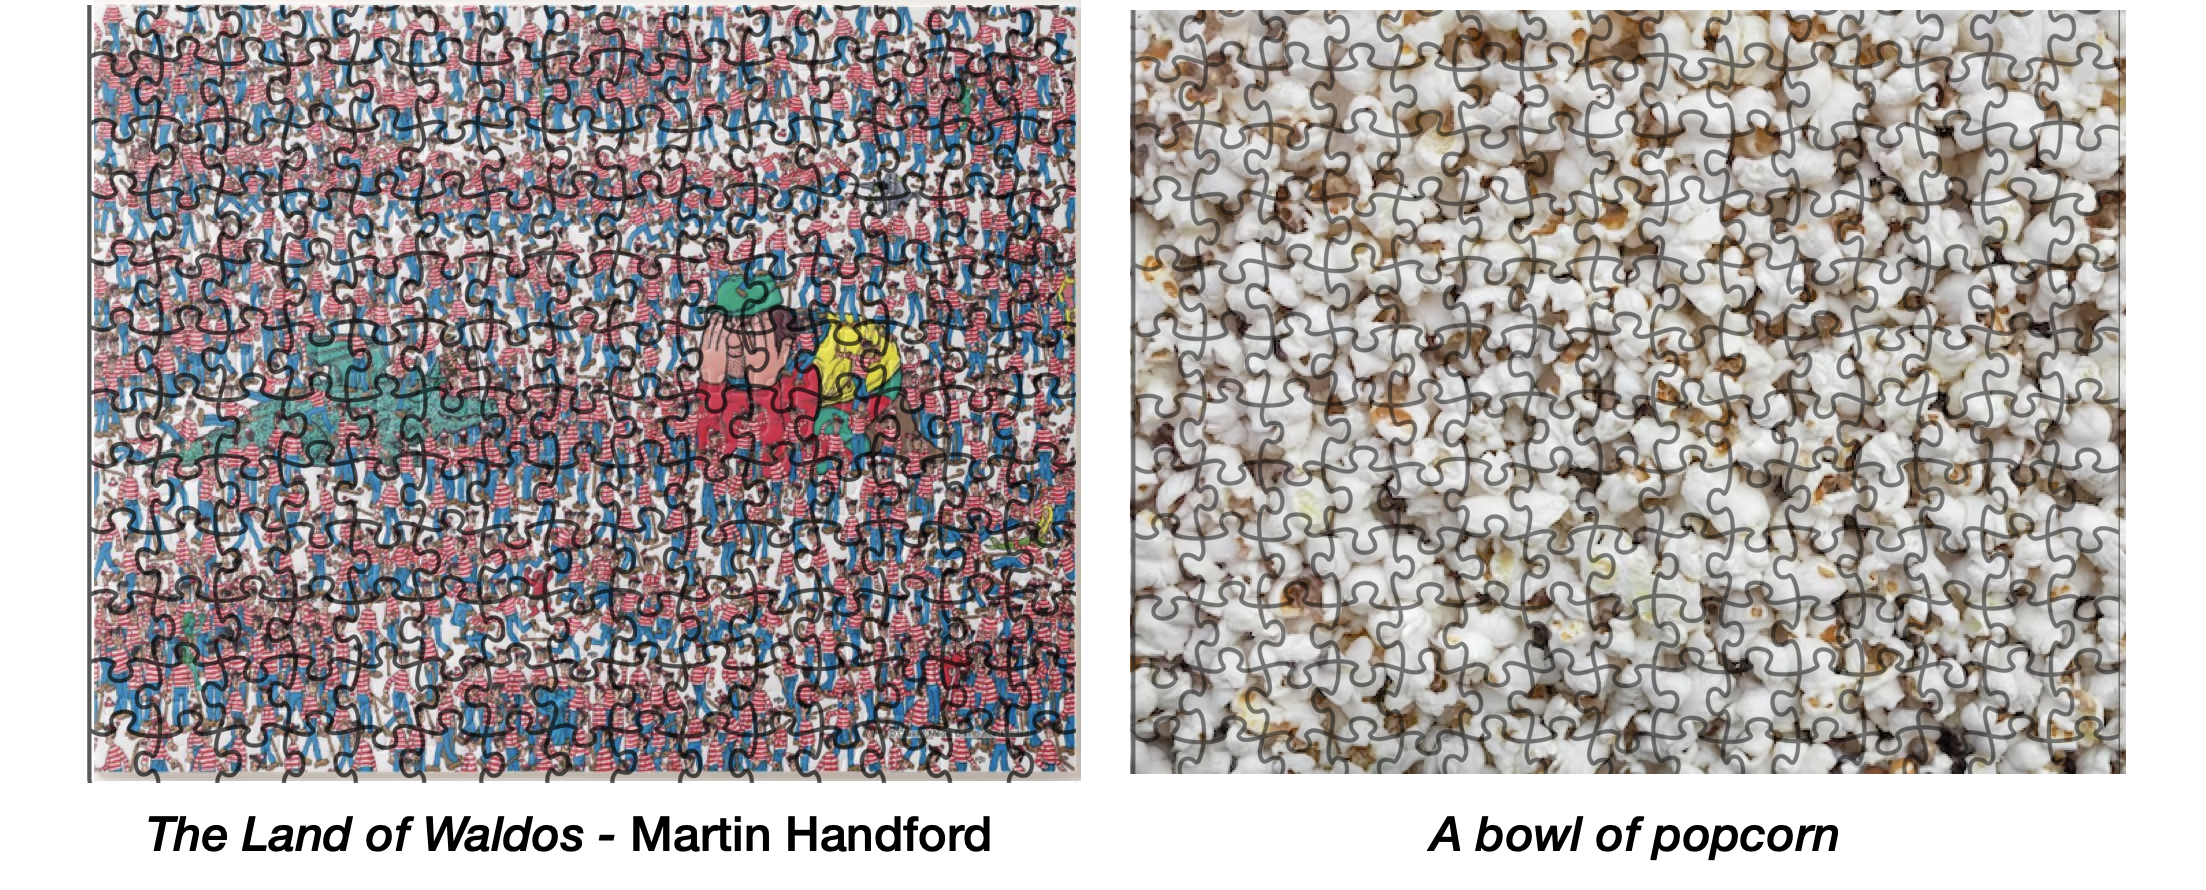
\includegraphics[width=\textwidth]{img/wallyVpopcorn}\\
Which of these jigsaw puzzles would be harder to solve? \\\pause Why?
\end{frame}


\begin{frame}
	\frametitle{Genome Sequencing}
	
		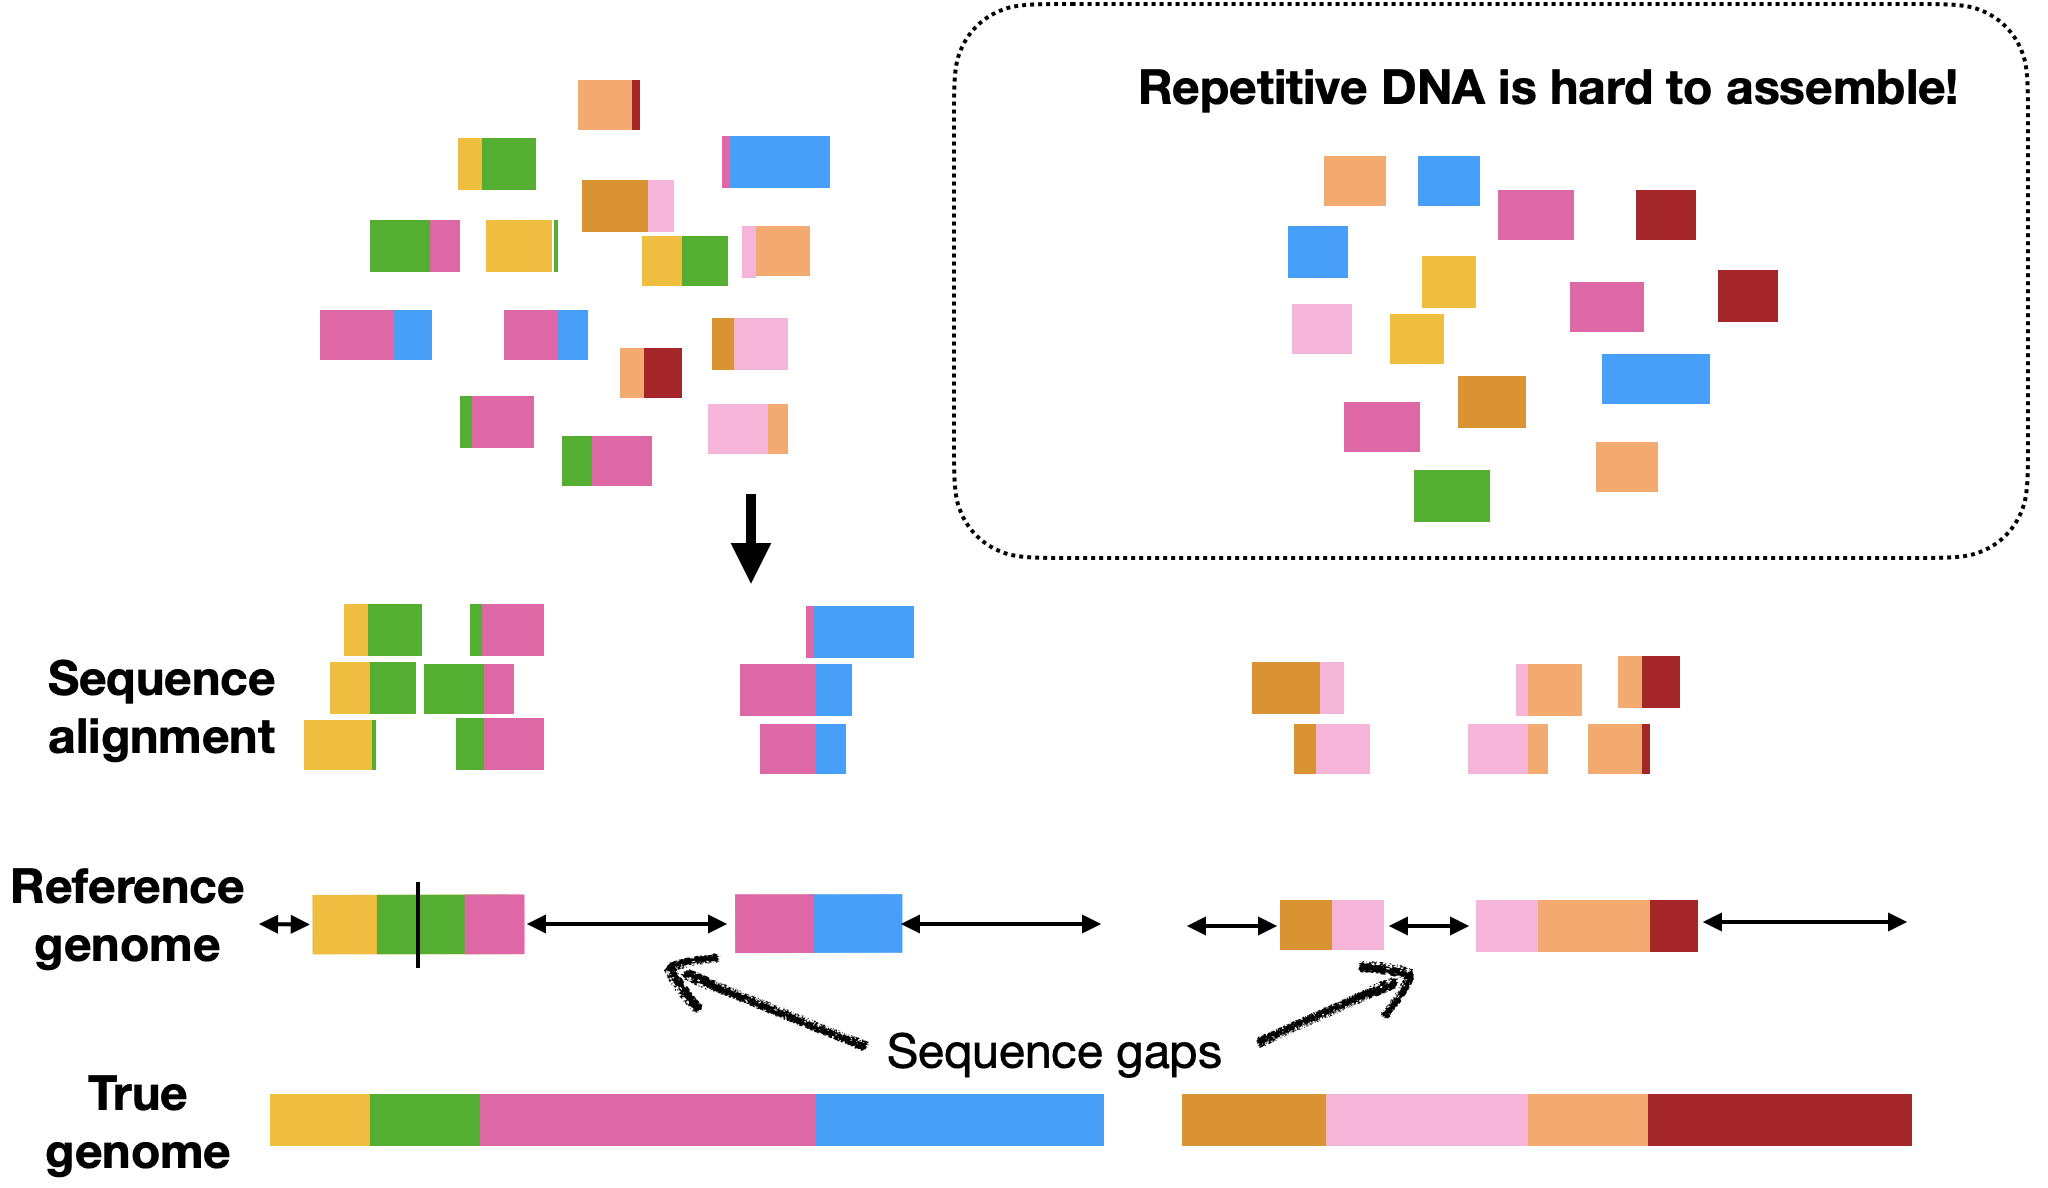
\includegraphics[width=\textwidth]{img/repetitiveDNAreference}
\end{frame}



\begin{frame}
	\center		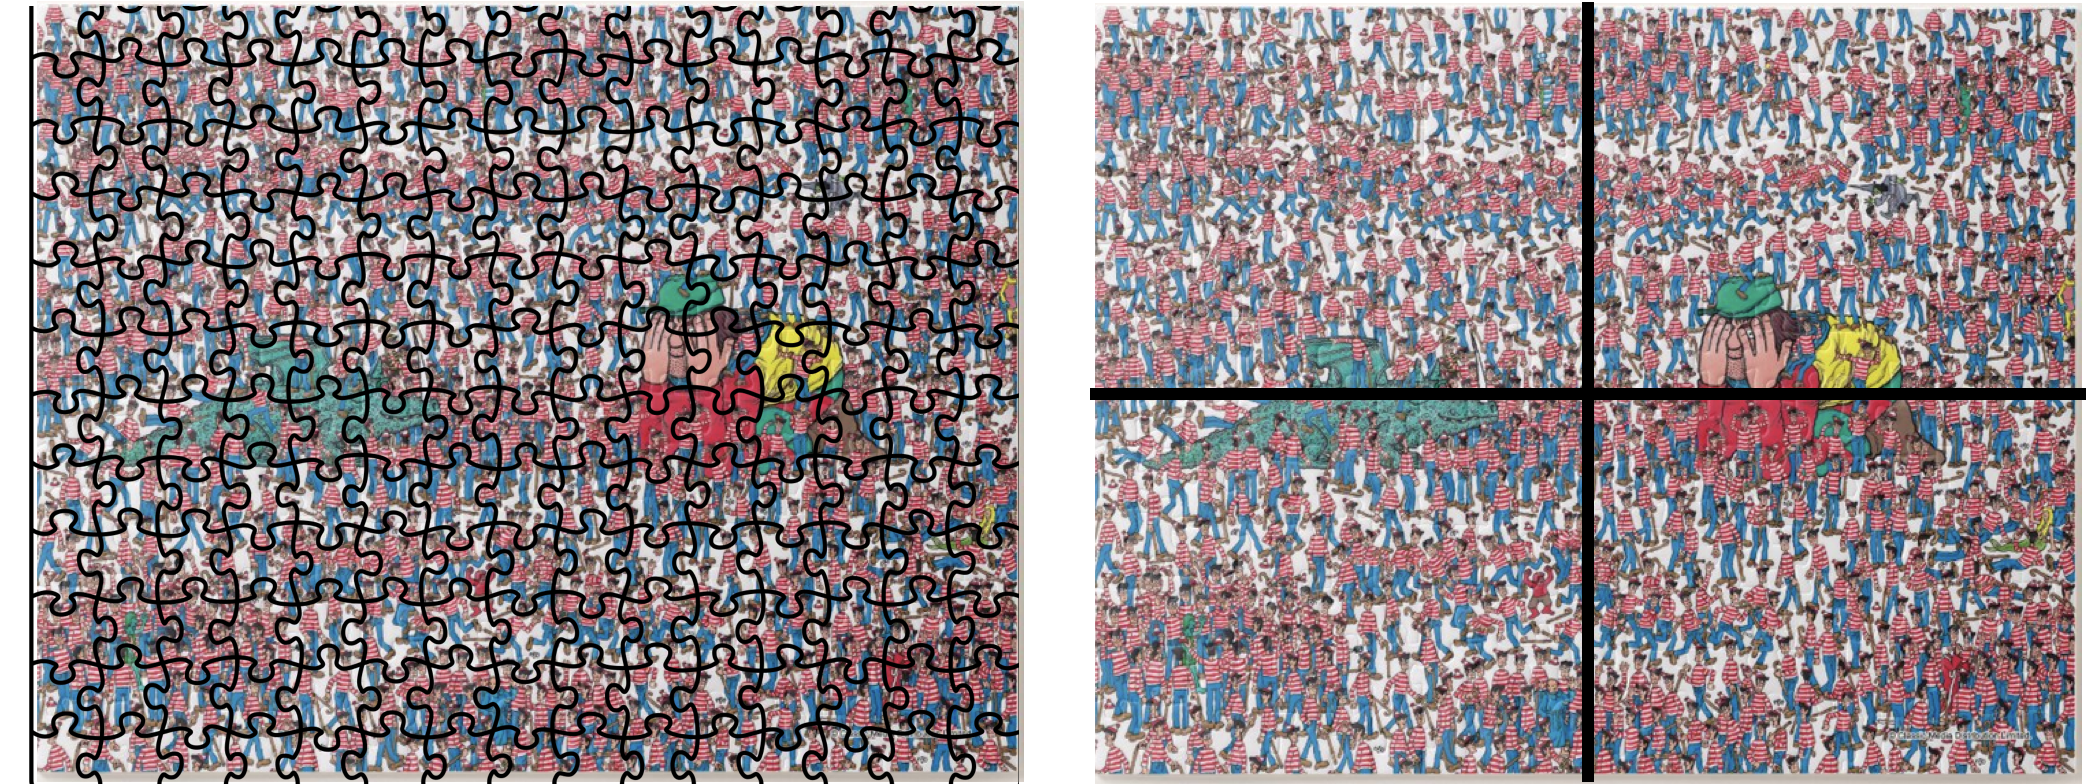
\includegraphics[width=\textwidth]{img/waldoBigpiece}\\
	Why is it easier to solve the puzzle on the right? \\
	\pause
	Puzzles with fewer, larger pieces are easier to solve!
\end{frame}


\begin{frame}
	\frametitle{Genome Sequencing - Long Reads}
	
	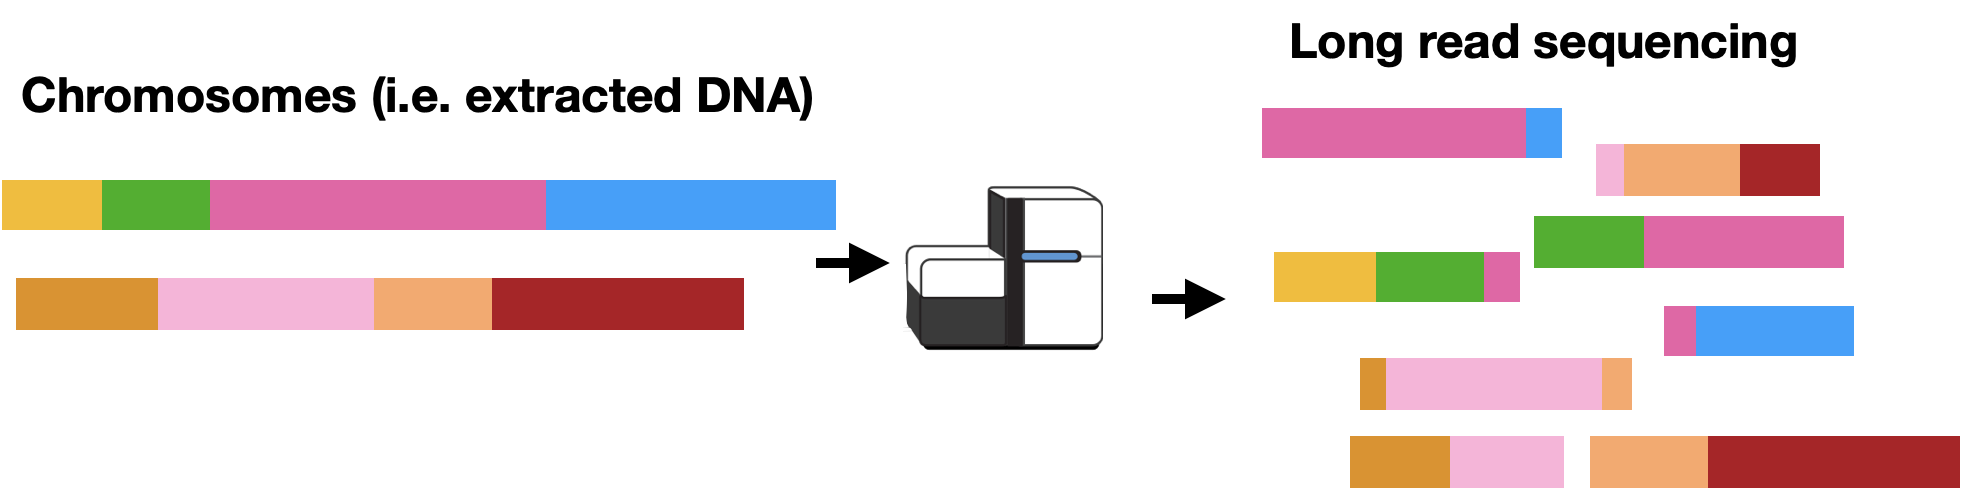
\includegraphics[width=\textwidth]{img/longReads}
\end{frame}


\begin{frame}
	\frametitle{Genome Sequencing - Long Reads}
	Longer reads improve assembly quality as they are more likely to span repetitive regions!
	\vspace{20pt}
	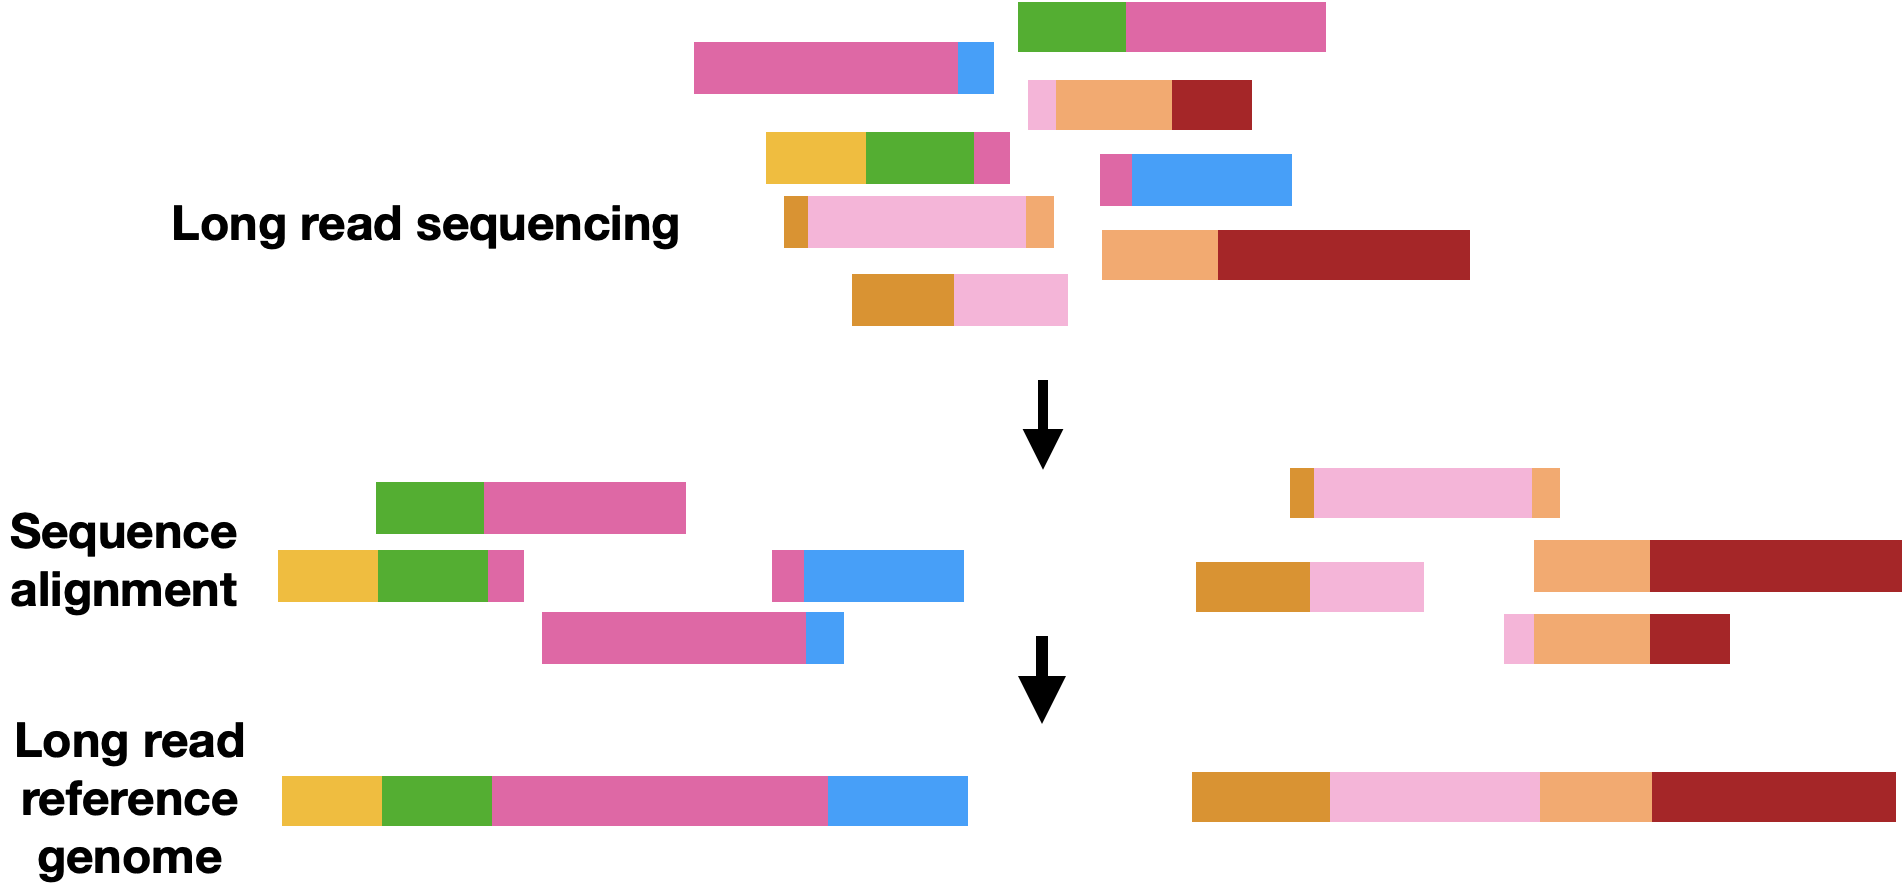
\includegraphics[width=\textwidth]{img/longReadAssembly}
\end{frame}


\begin{frame}
	\frametitle{Genome Sequencing - Long Read Technologies}
\centering 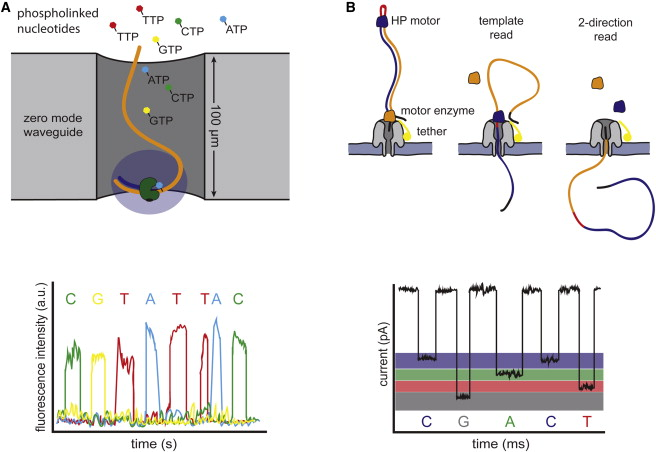
\includegraphics[width=0.7\textwidth]{img/pacBioNanopore}
\begin{itemize}
	\item[\textbf{A}] PacificBioscience's SMRT sequencing
	\item[\textbf{B}] Oxford Nanopore sequencing
\end{itemize}
\blfootnote{Image from: Reuter et al 2015 - \textit{Molecular Cell}}
\end{frame}


\begin{frame}
	\frametitle{Genome Sequencing - Sequencers}
\centering \includegraphics[width=\textwidth]{img/sequencers}
\blfootnote{You don't have to memorize the names!}
\end{frame}


\begin{frame}
	\frametitle{Genome Sequencing - Short vs Long Reads}

		Longer reads improve assembly quality as they are more likely to span repetitive regions!\\
		\vspace{10pt}
		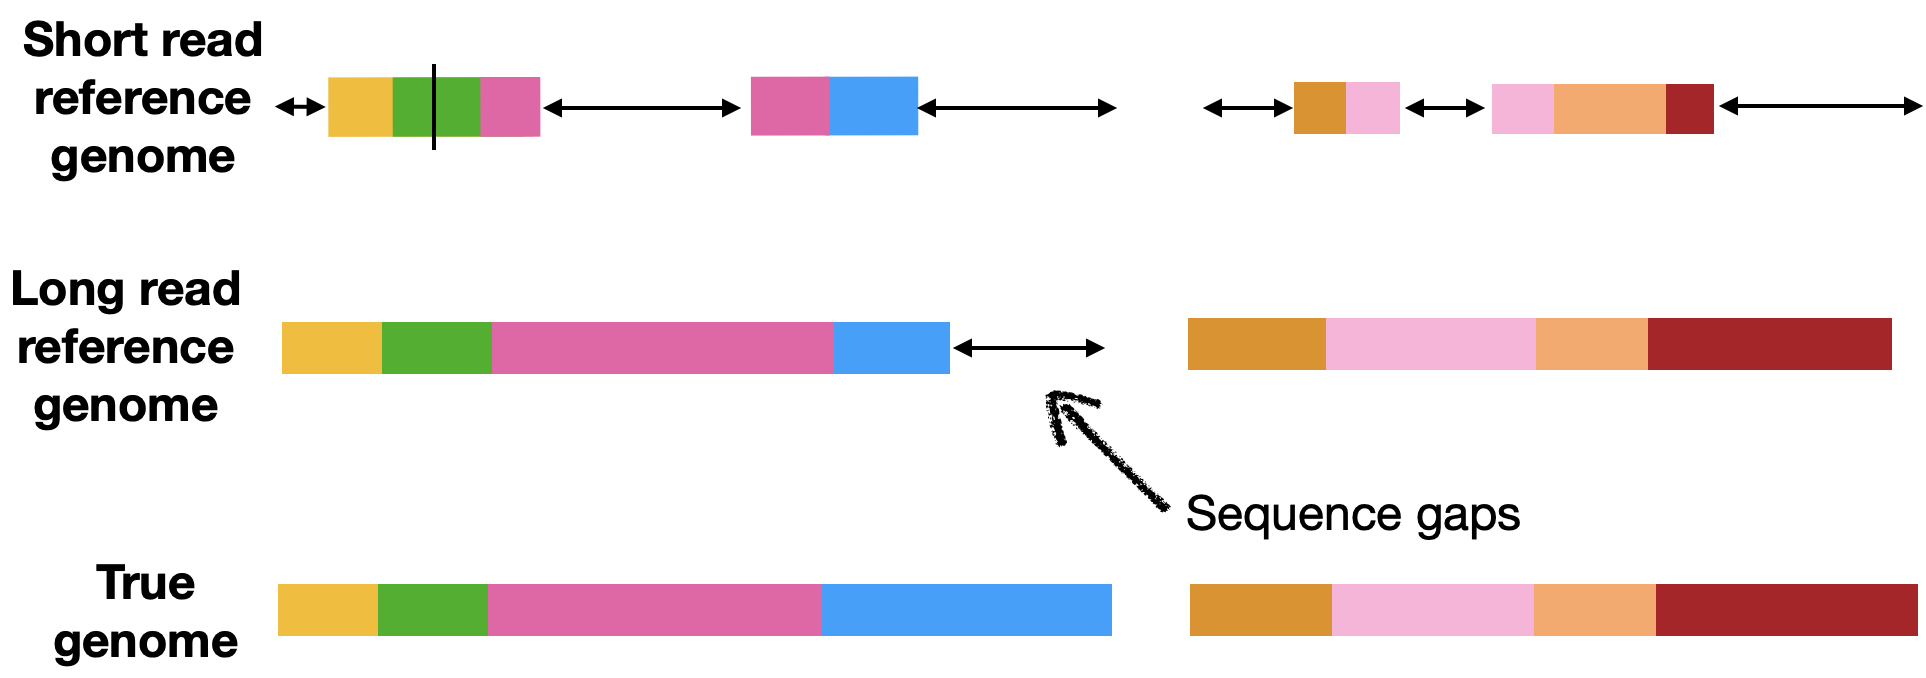
\includegraphics[width=\textwidth]{img/referenceGenomeComparison}
		\pause
		\centering{So why use short reads?}
\end{frame}

\begin{frame}
	\frametitle{Genome Sequencing - Different approaches}
	
Different sequencing methodologies have their uses in different settings\\
	
\begin{tabular}{|r|c|c|c|c|}
\hline
	&\thead{Sanger\\ sequencing}& \thead{Illumina\\(Short-reads)} & \thead{PacBio\\(long-reads)} &  \thead{ONT\\Nanopore\\(long-reads)}\\
	\hline
	Cost & --- & +++ & - & + \\
	Accuracy & +++ & ++ & +  & 0 \\ 
	Assembly & - & - & +++ & ++ \\
	Computation & --- & - & ++ & ++ \\
	\hline
\end{tabular}
\blfootnote{The above table related to the applicability of the different methods for genome assembly}
\end{frame}


\begin{frame}
	
	\Huge
	Questions? \\ \pause
	Let's take a short break
	
\end{frame}


\begin{frame}
			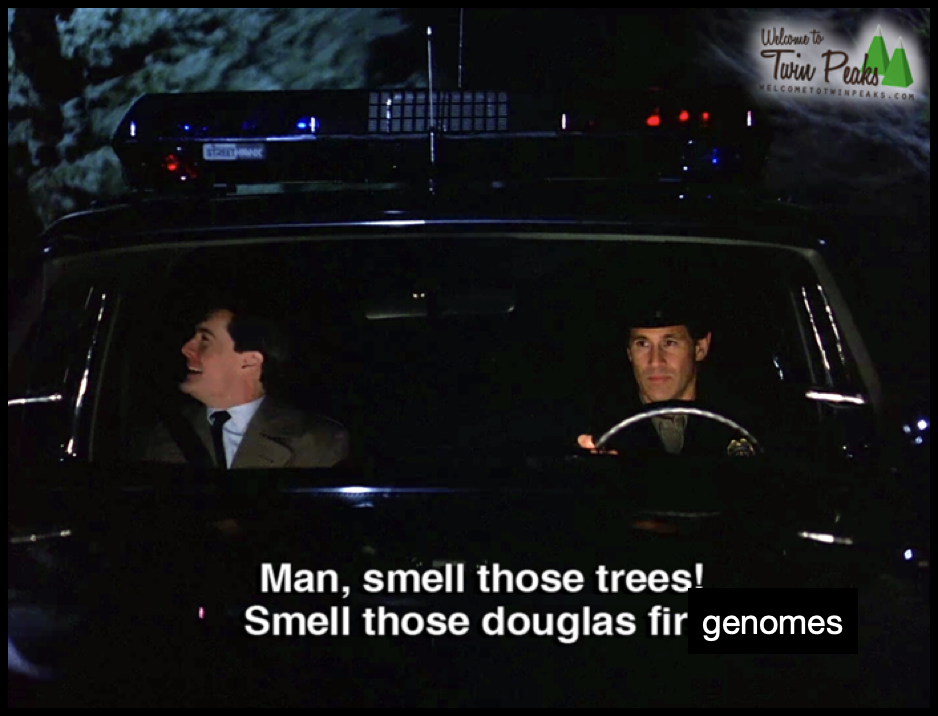
\includegraphics[width=\textwidth]{img/cooper}
	\end{frame}
	



\begin{frame}
	\frametitle{Conifer genomes}
	
	Conifer species have clear ecological and cultural importance\\
		
	Fundamental to forestry in Canada\\
	
% The unicode characters for the indiginous names were really finnicky, so I just copied them from Keynote  - don't tell anyone
			\centering	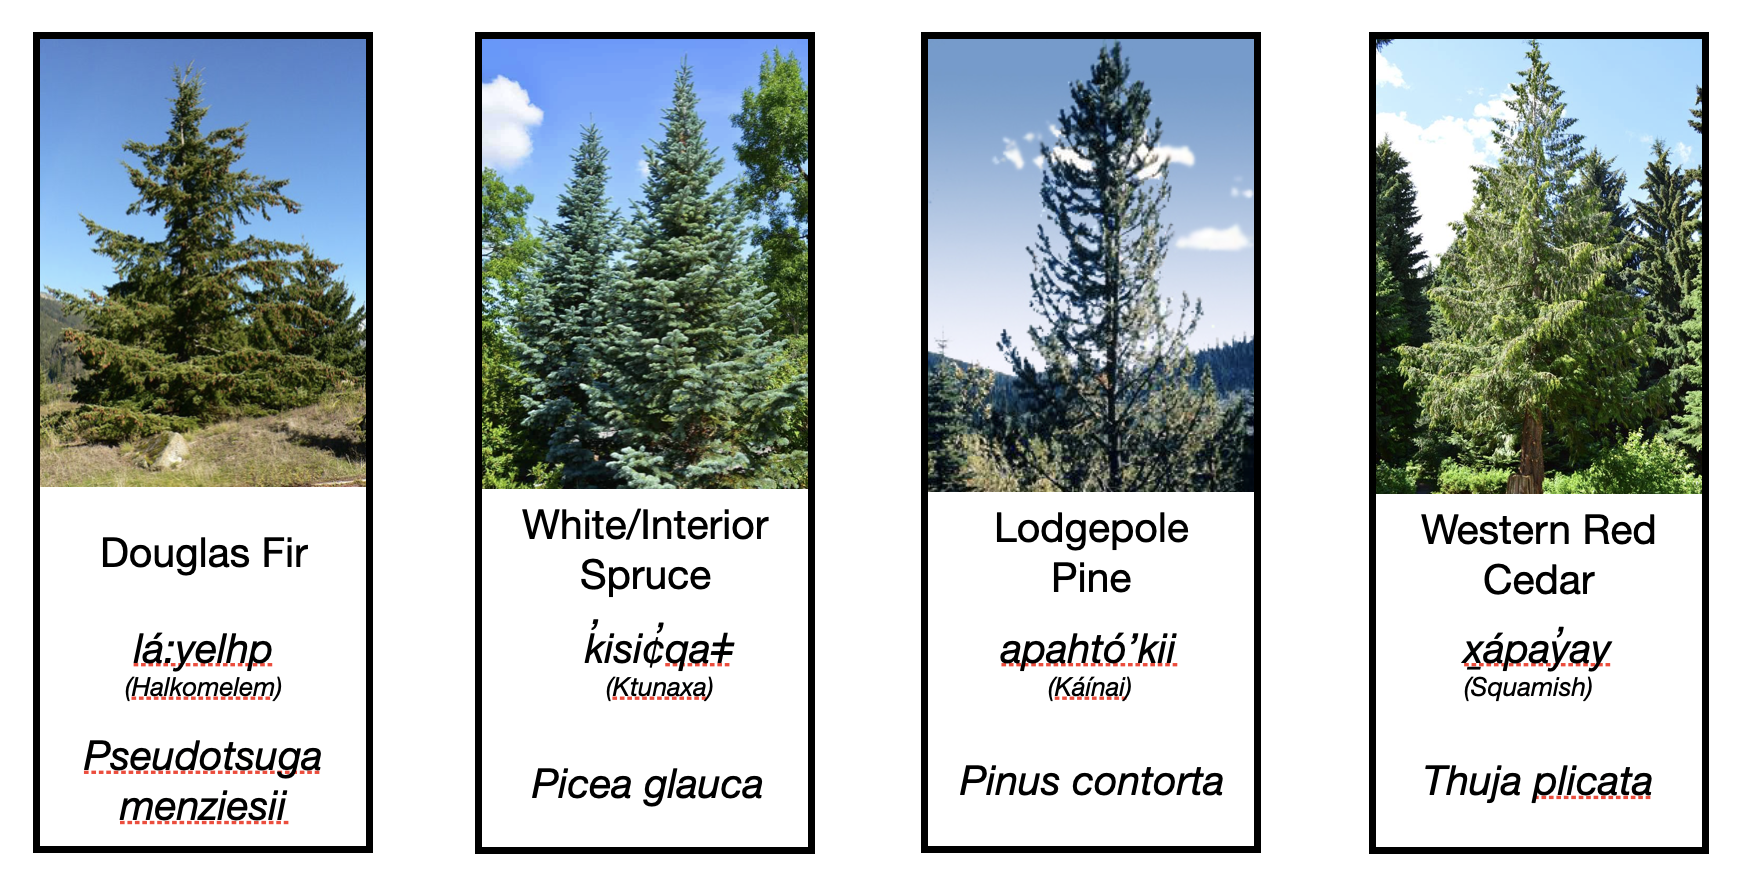
\includegraphics[keepaspectratio, width  =1\textwidth]{img/conifers}\\

%\small \centering \textit{\textbf{The smallest of these is still $>$ 3x larger than the human genome!}}
	
\end{frame}


\begin{frame}
\frametitle{Genome Sizes}
			\centering	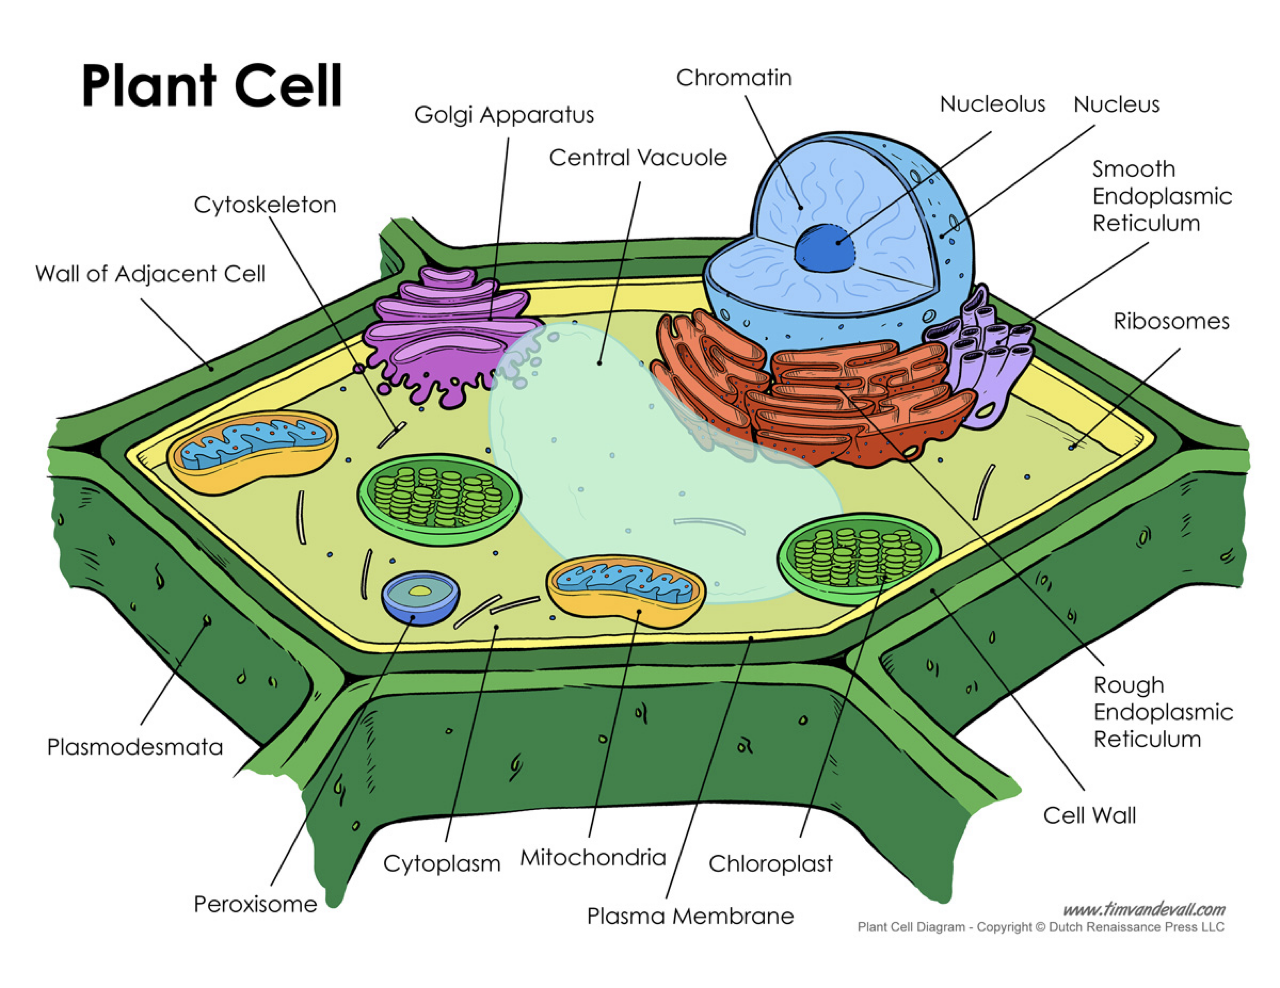
\includegraphics[keepaspectratio, width  =1\textwidth]{img/plantCell}\\
\end{frame}
	

\begin{frame}
	\frametitle{Genome Sizes}
	\centering	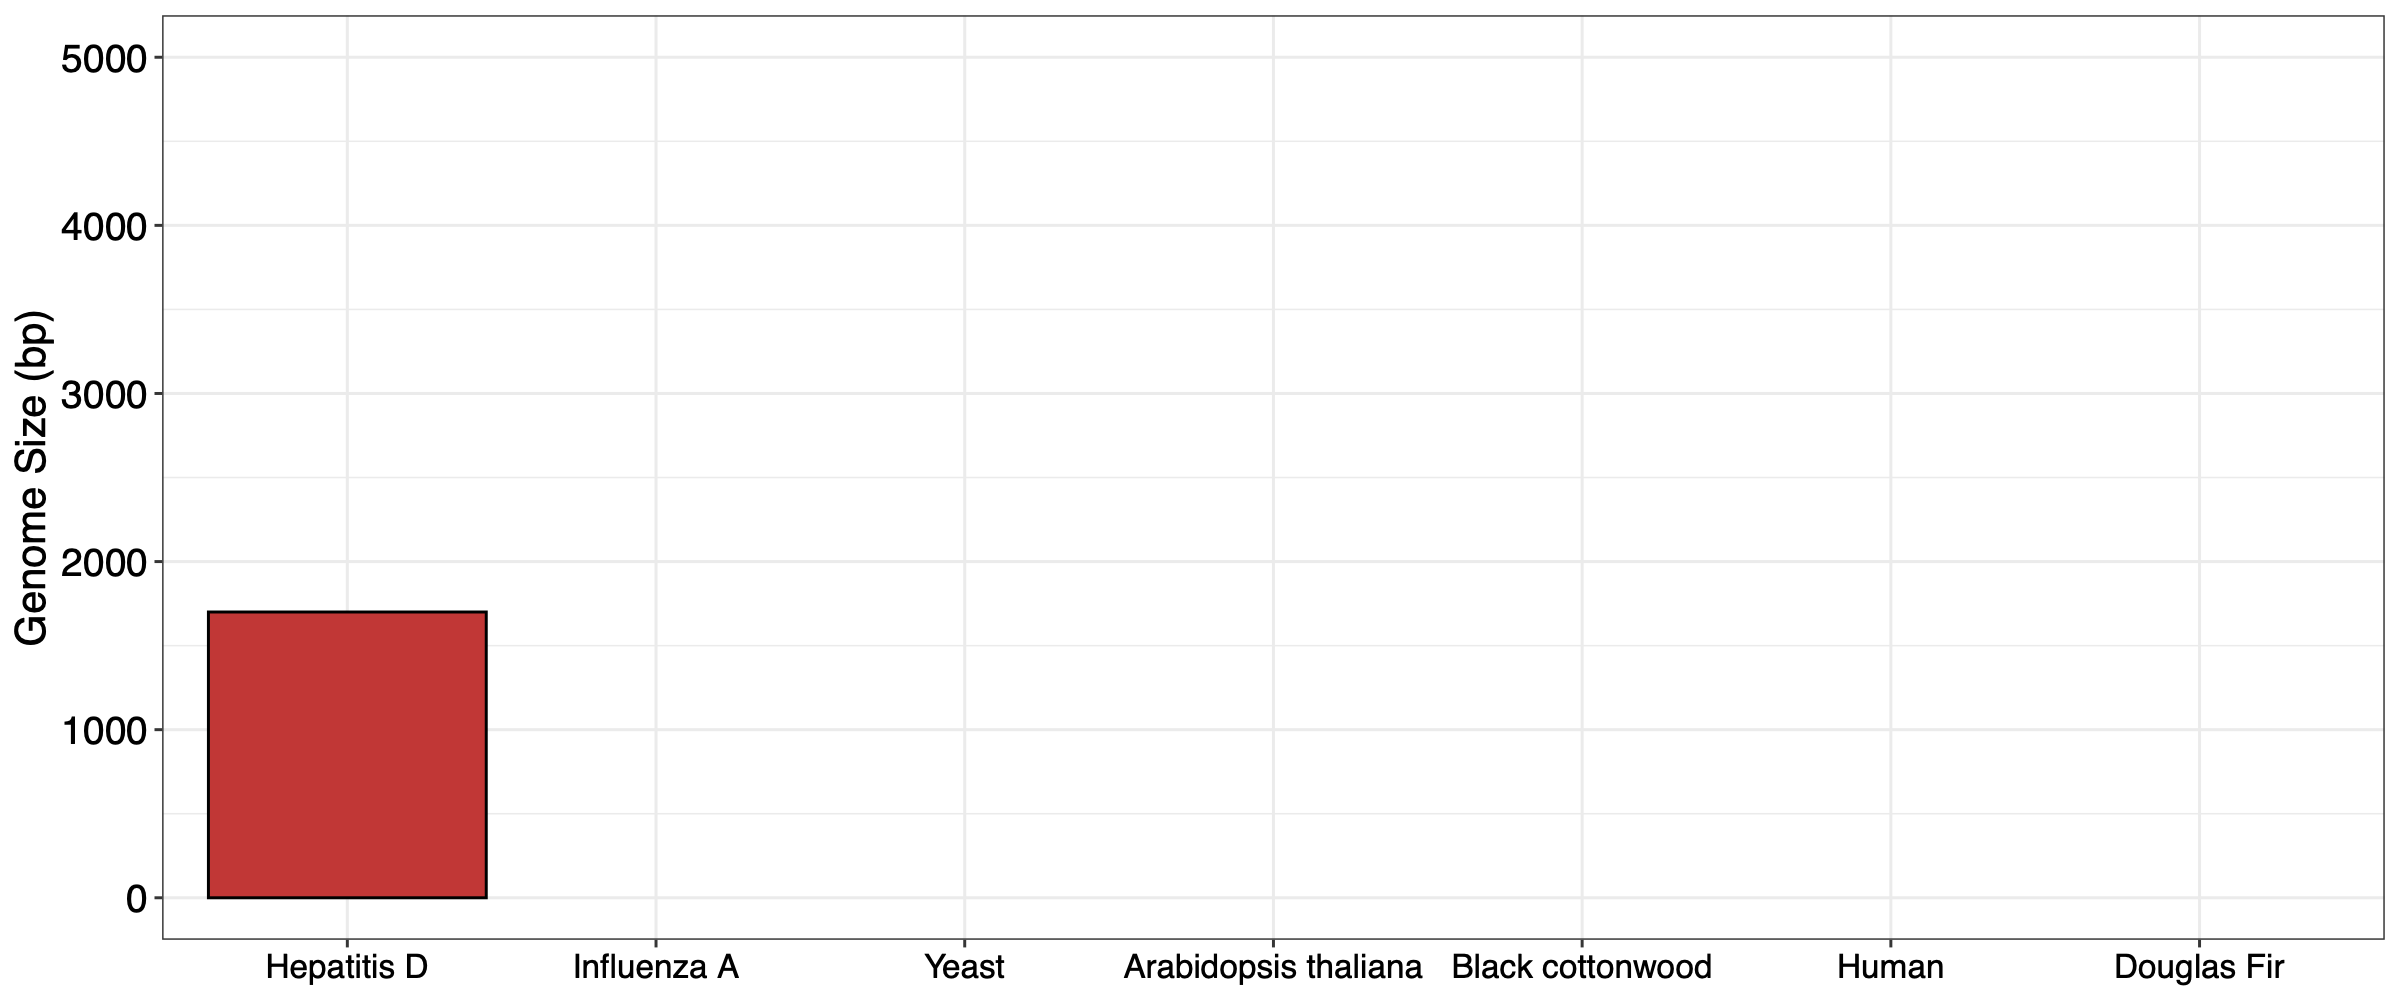
\includegraphics[keepaspectratio, width  =1\textwidth]{img/hepD.png}\\
\end{frame}

\begin{frame}
	\frametitle{Genome Sizes}
	\centering	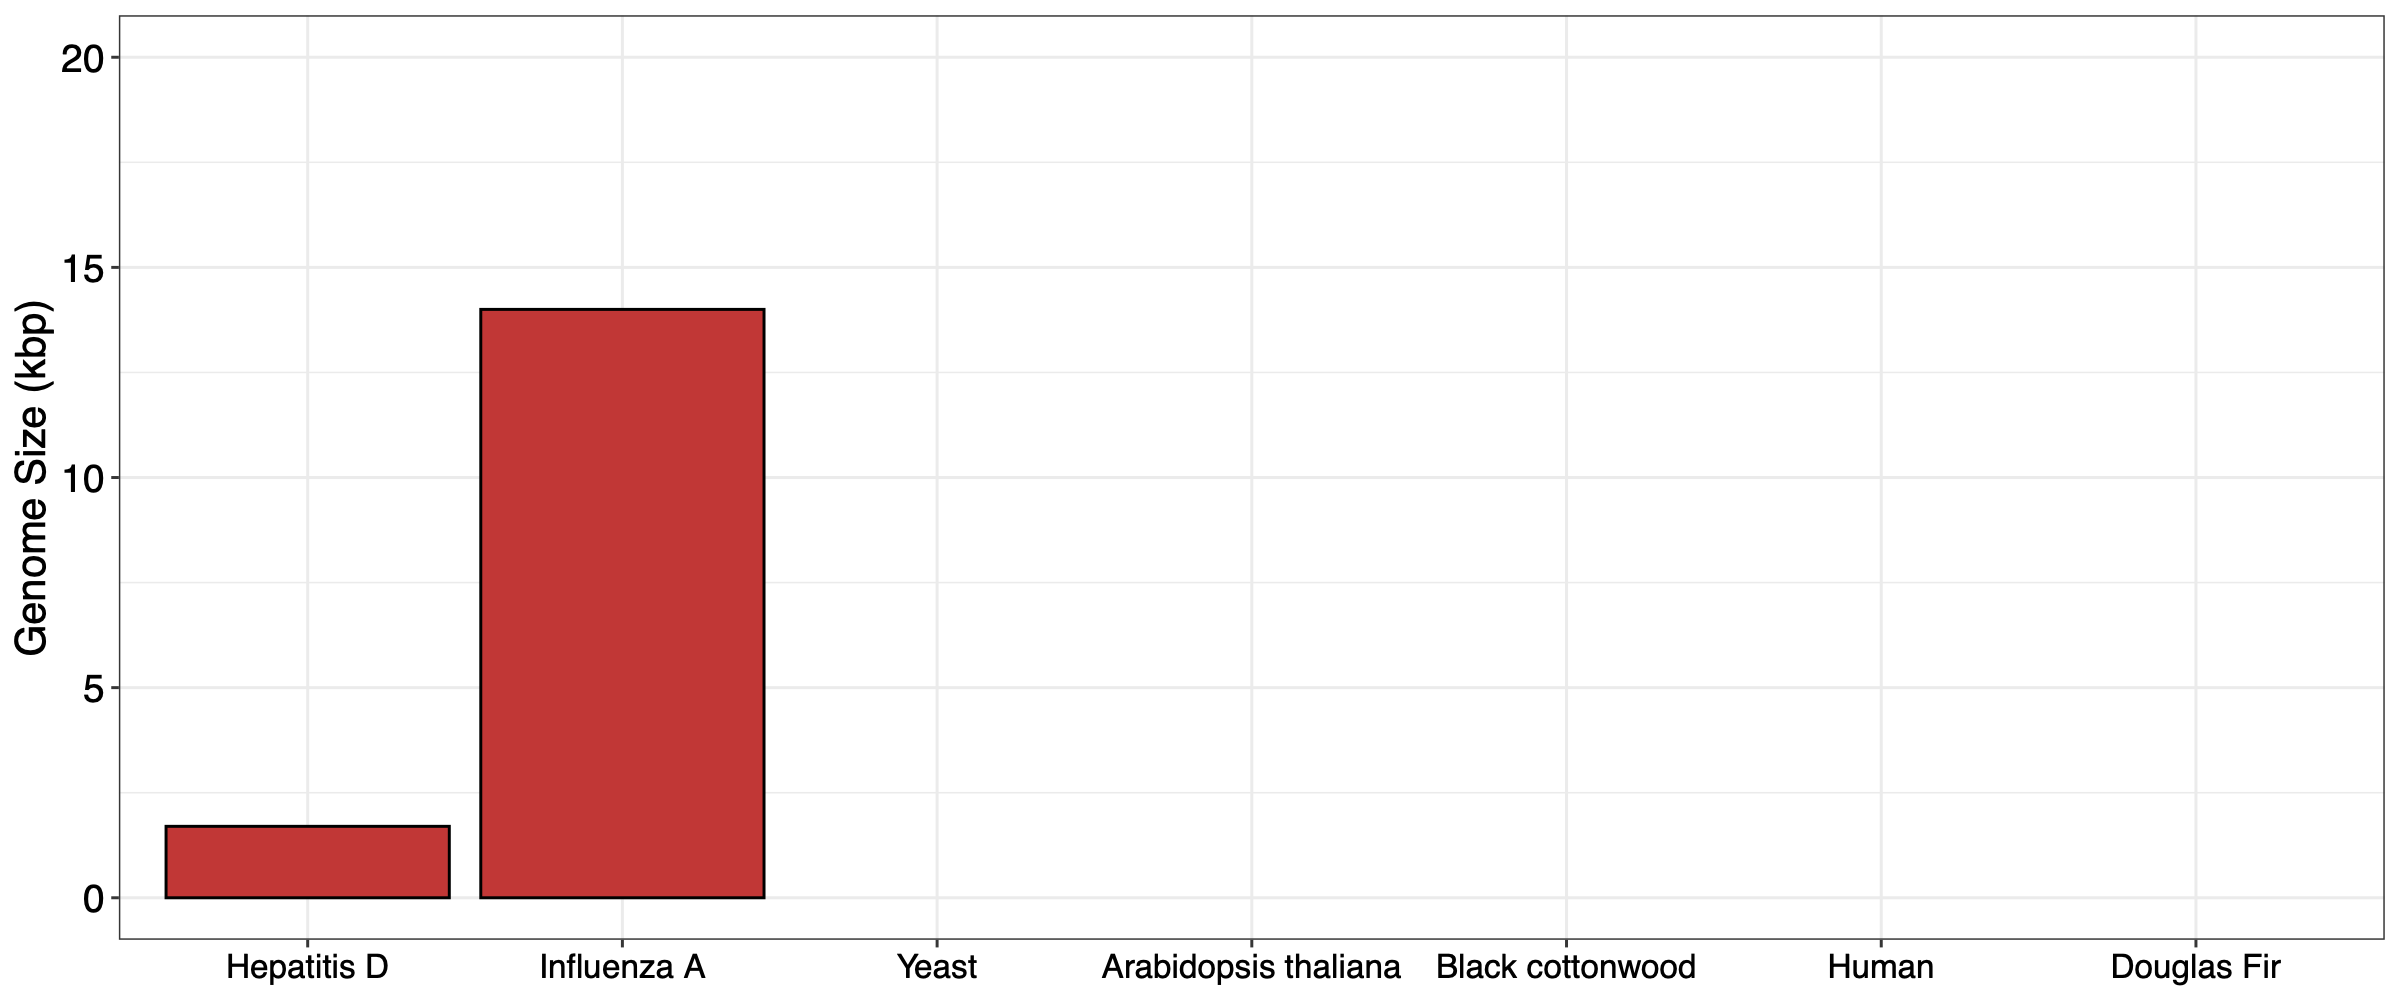
\includegraphics[keepaspectratio, width  =1\textwidth]{img/flu.png}\\
\end{frame}

\begin{frame}
	\frametitle{Genome Sizes}
	\centering	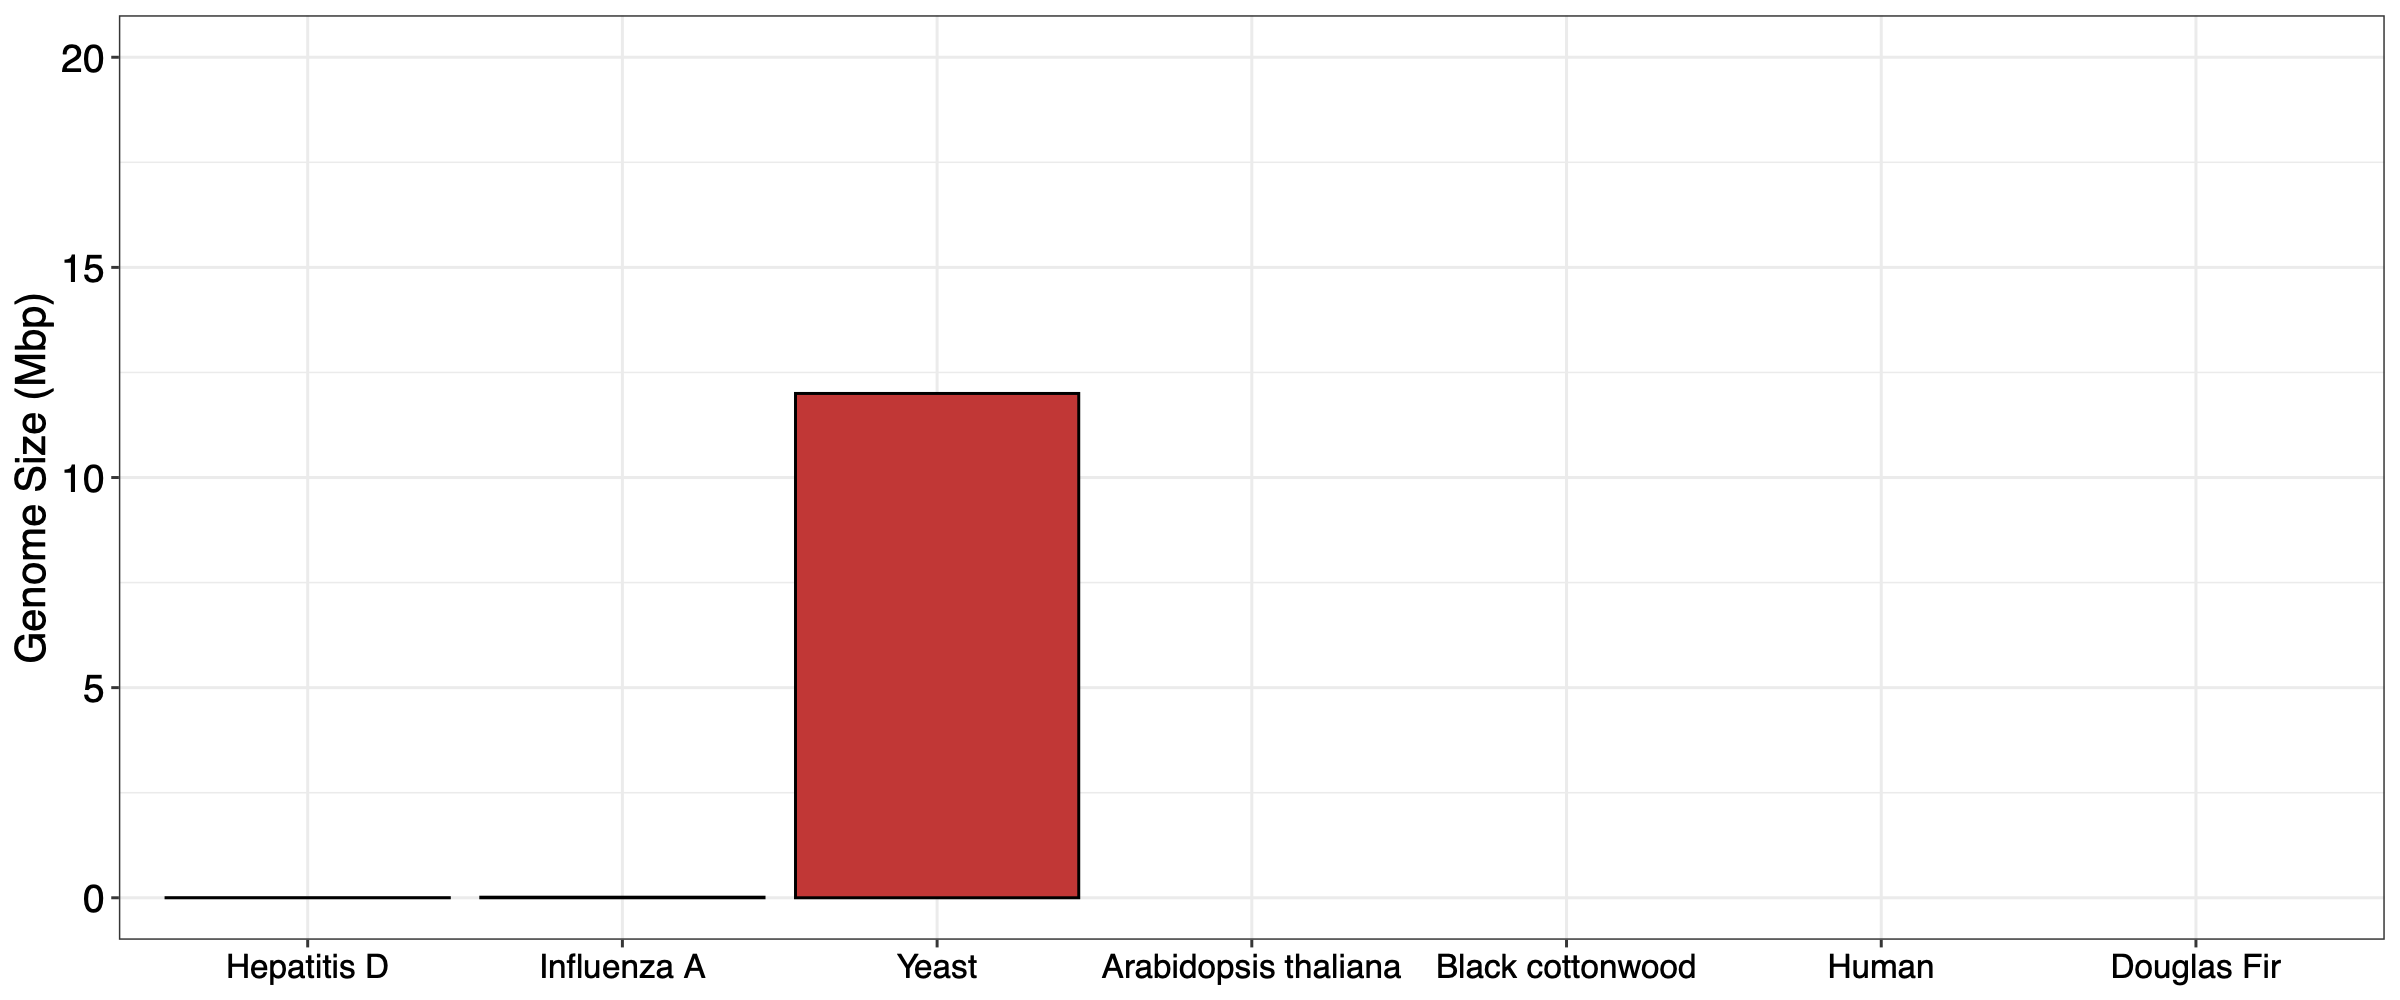
\includegraphics[keepaspectratio, width  =1\textwidth]{img/yeast.png}\\
\end{frame}

\begin{frame}
	\frametitle{Genome Sizes}
	\centering	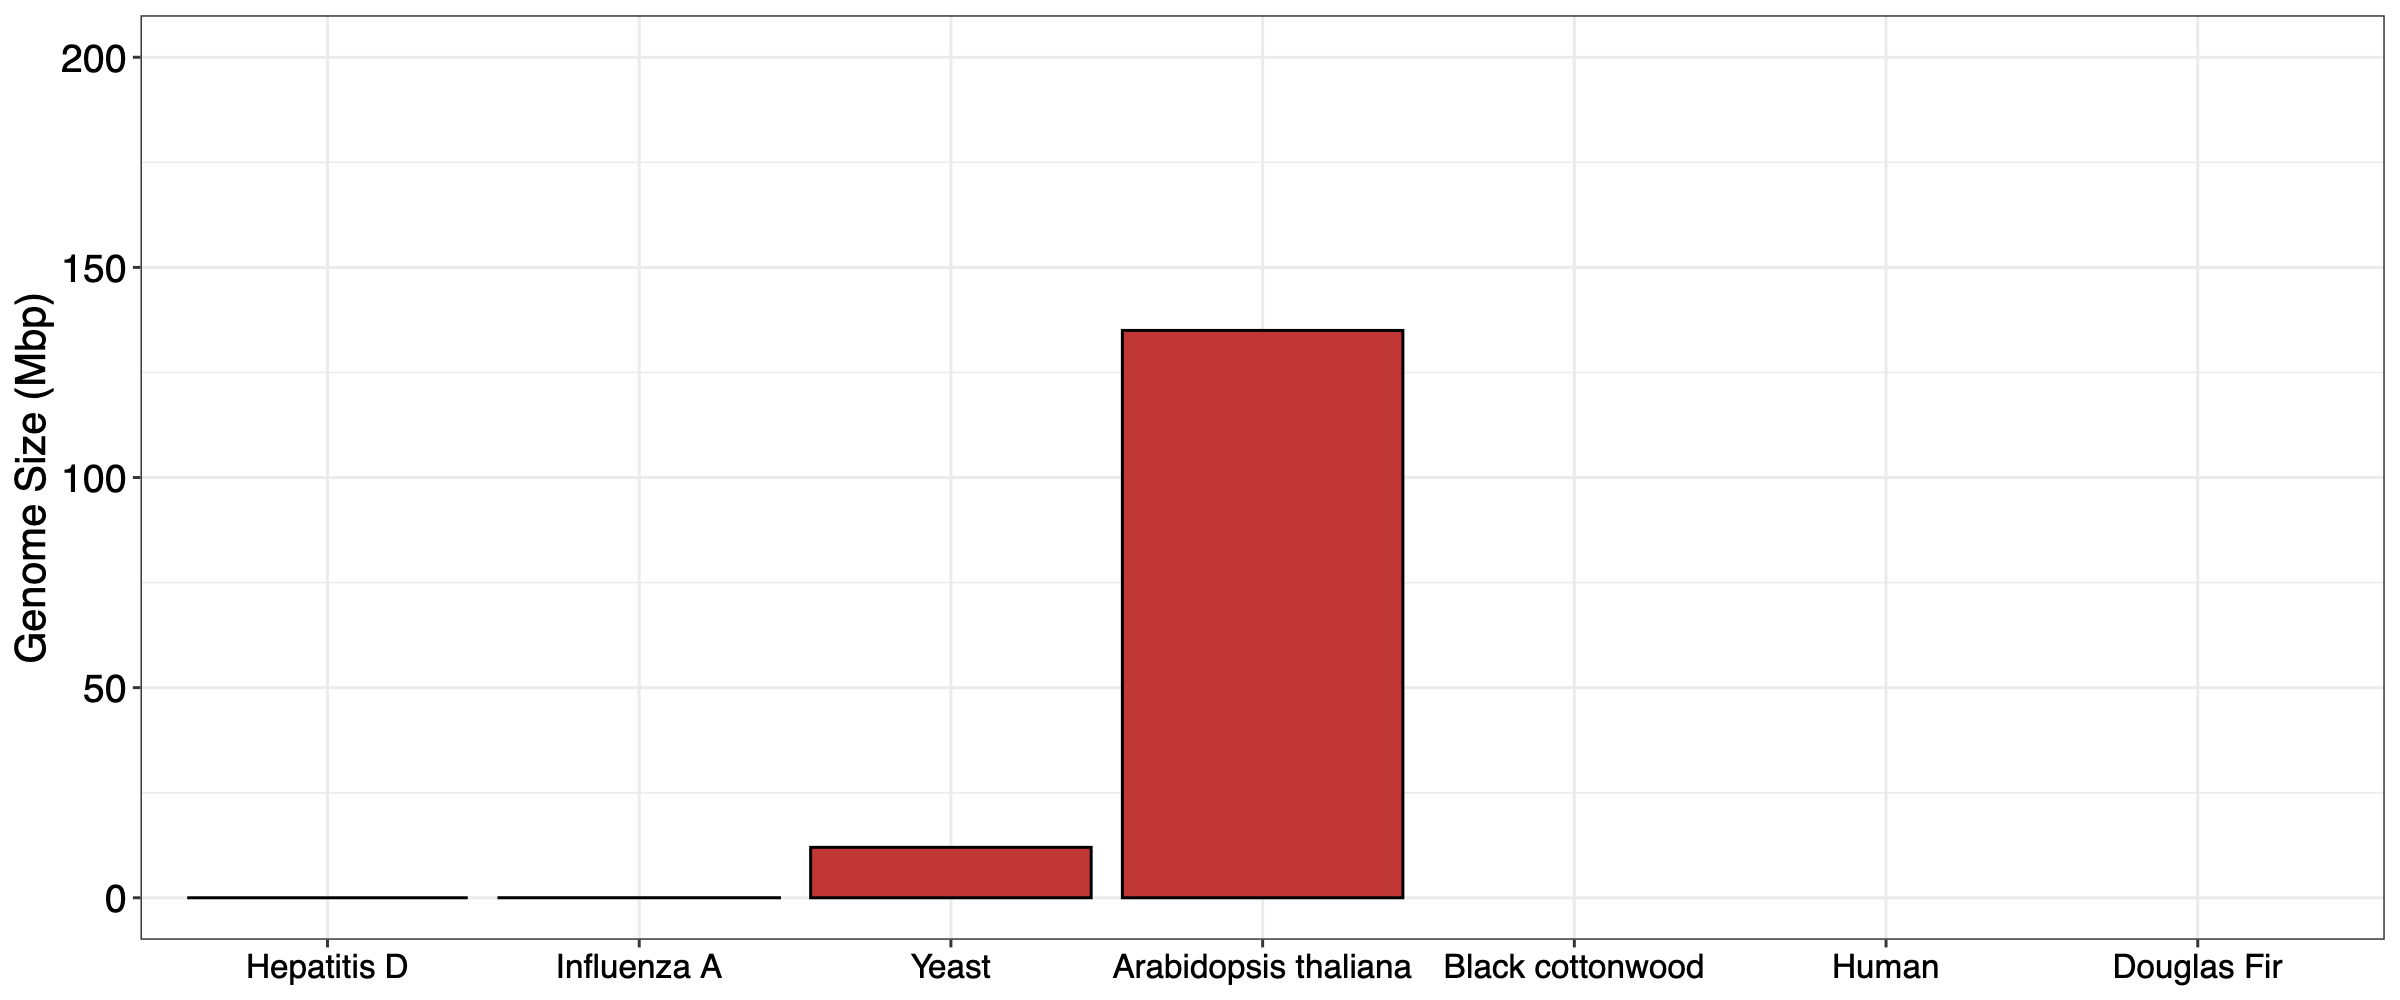
\includegraphics[keepaspectratio, width  =1\textwidth]{img/arabidopsis.png}\\
\end{frame}

\begin{frame}
	\frametitle{Genome Sizes}
	\centering	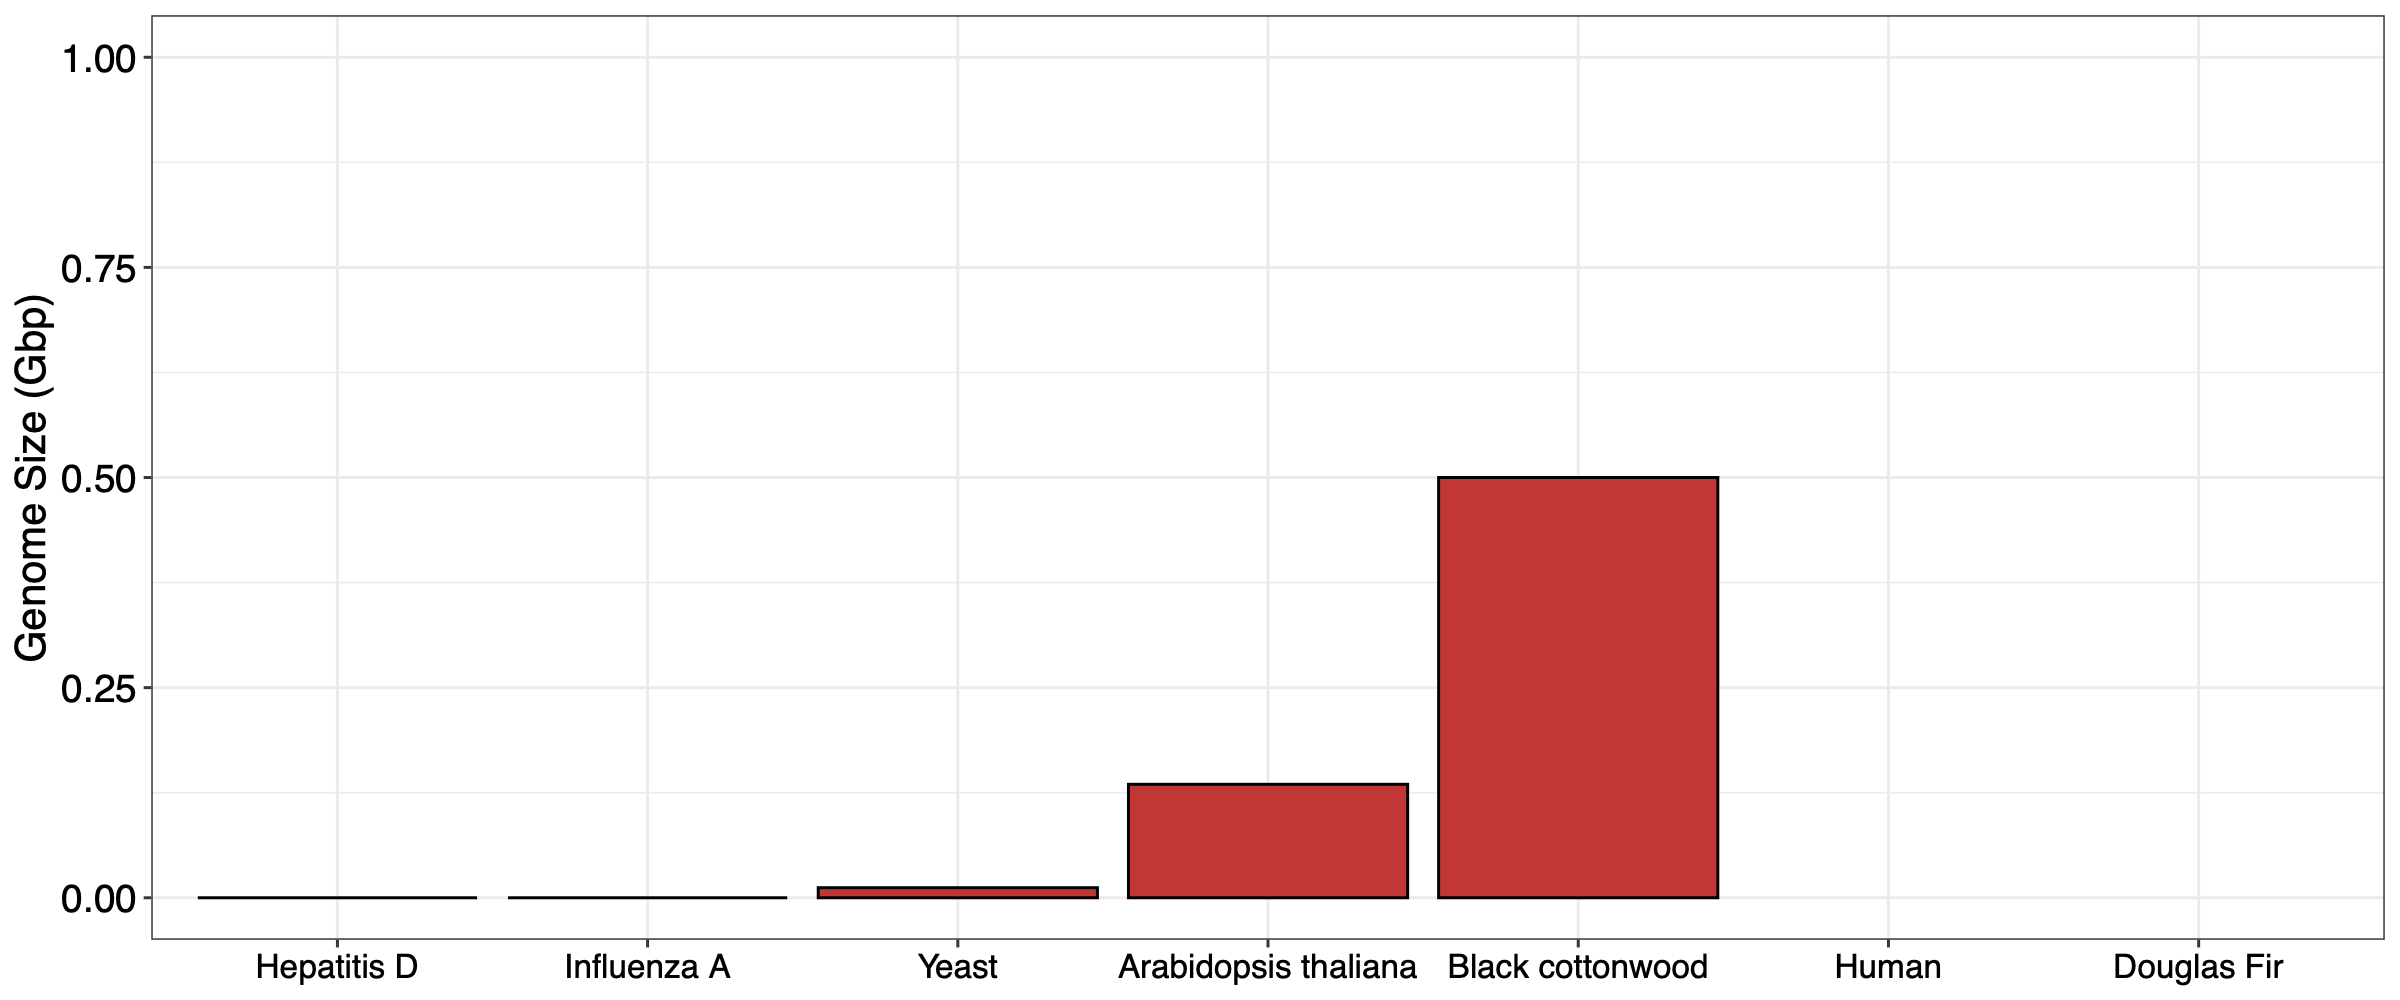
\includegraphics[keepaspectratio, width  =1\textwidth]{img/cottonwood.png}\\
\end{frame}

\begin{frame}
	\frametitle{Genome Sizes}
	\centering	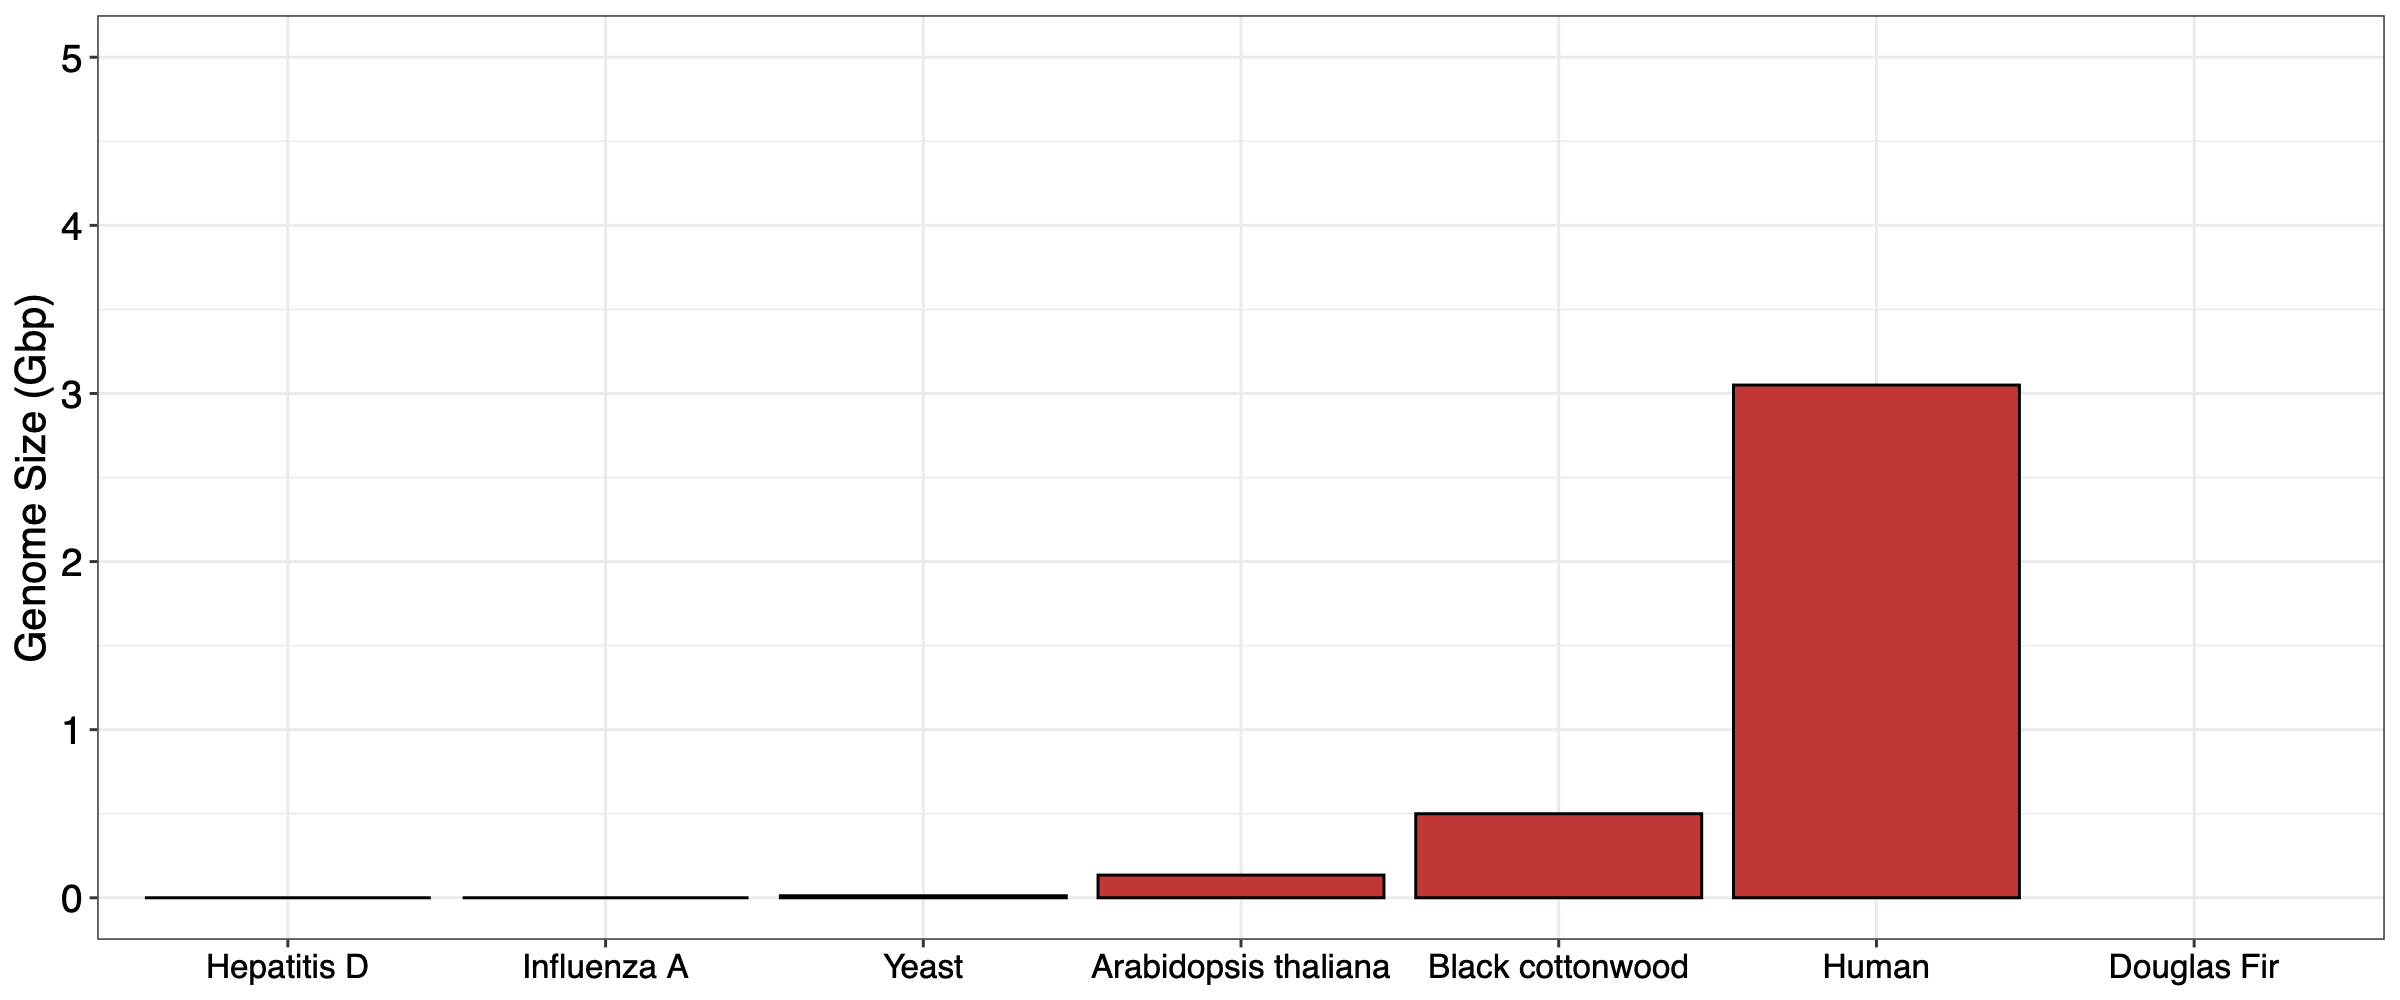
\includegraphics[keepaspectratio, width  =1\textwidth]{img/human.png}\\
\end{frame}



\begin{frame}
	\frametitle{Genome Sizes}
	\centering	\includegraphics[keepaspectratio, width  =1\textwidth]{img/dougFir.png}\\
	\vspace{10pt}
	Every cell of a Douglas-fir contains more than $5x$ the DNA than any human cell!

\blfootnote{As with ploidy and chromosome count, DNA volume is not a good predictor of an organism's complexity} 
\end{frame}

\begin{frame}
	\frametitle{Genome Sizes - Conifers}
	\centering	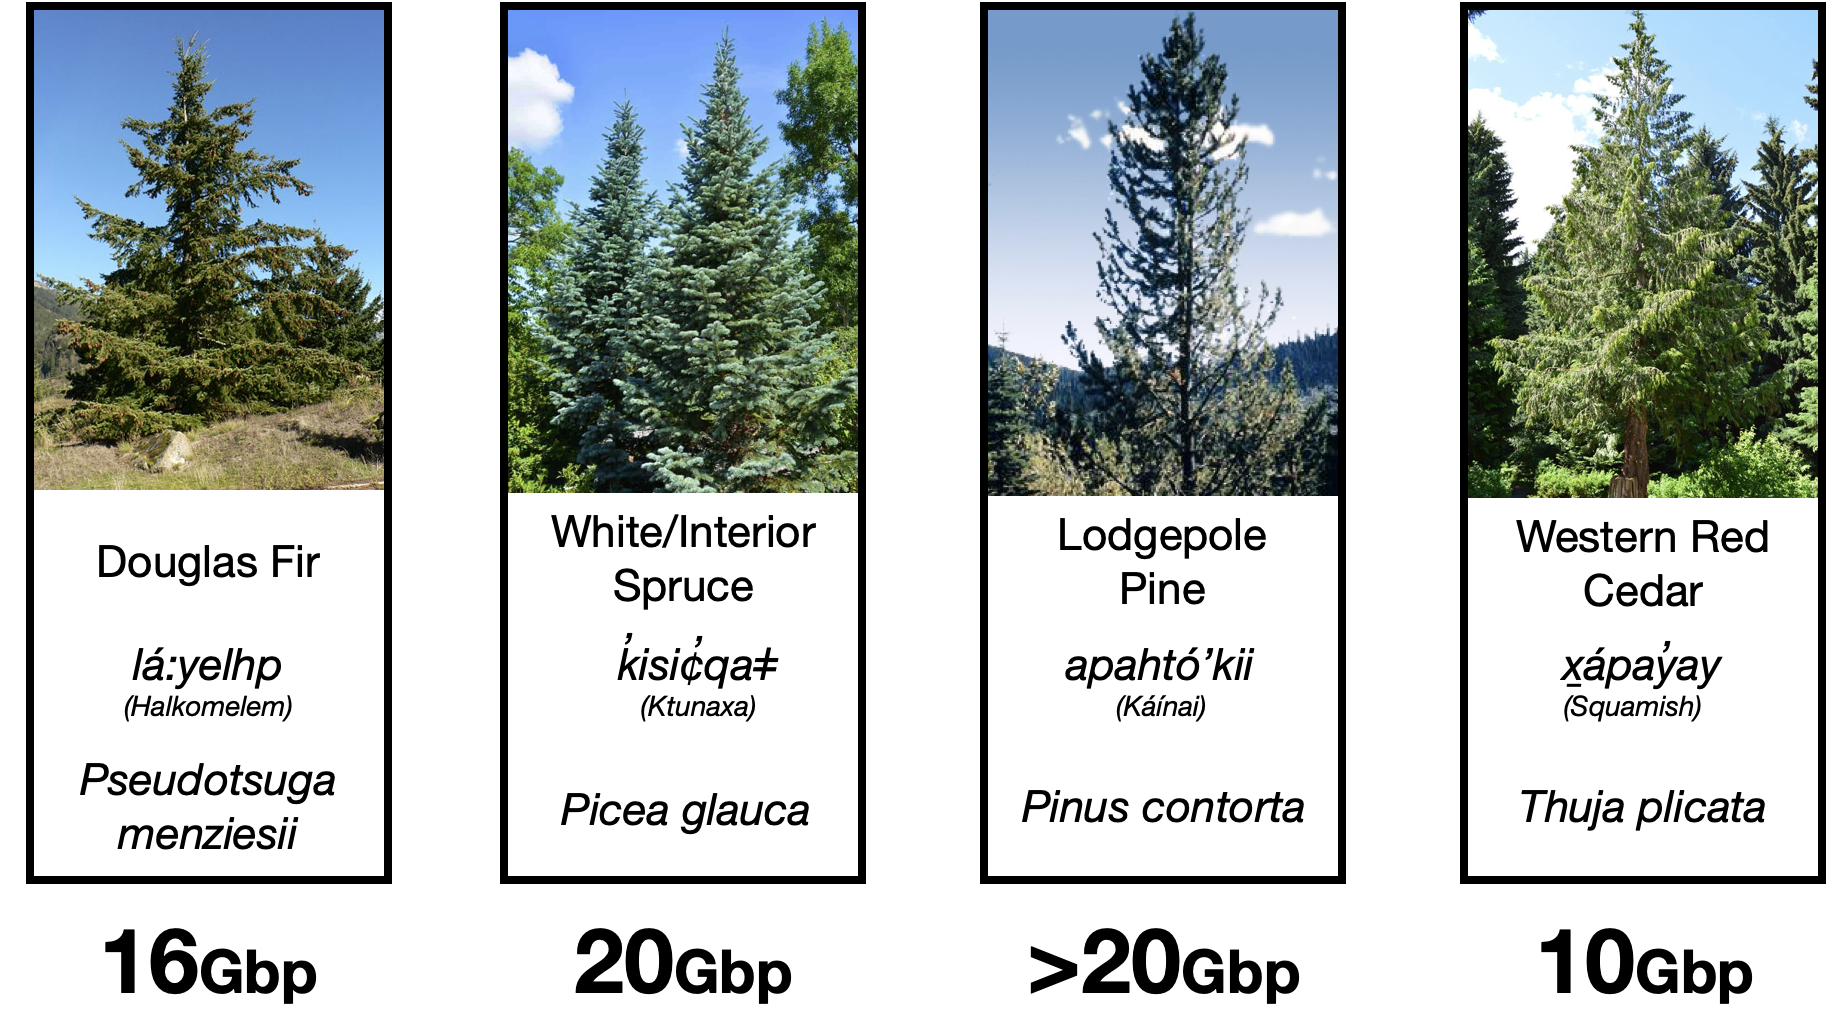
\includegraphics[keepaspectratio, width  =1\textwidth]{img/conifersSize.png}\\
	\textbf{\textit{The smallest of these is still more than $3x$ the human genome!}}
\end{frame}



    {
	\usebackgroundtemplate{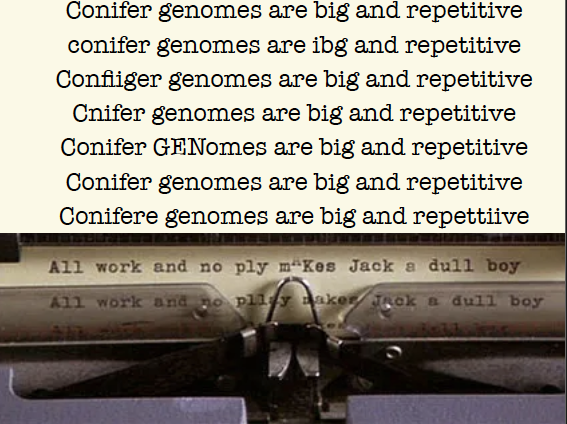
\includegraphics[height=\paperheight,width=\paperwidth]{img/genomes}}
	\setbeamertemplate{navigation symbols}{}
	\begin{frame}[plain]
	\end{frame}
}

\begin{frame}
	\frametitle{Print Out the Douglas-fir Genome}
	\begin{columns}
		\begin{column}{0.4\textwidth}
						\centering	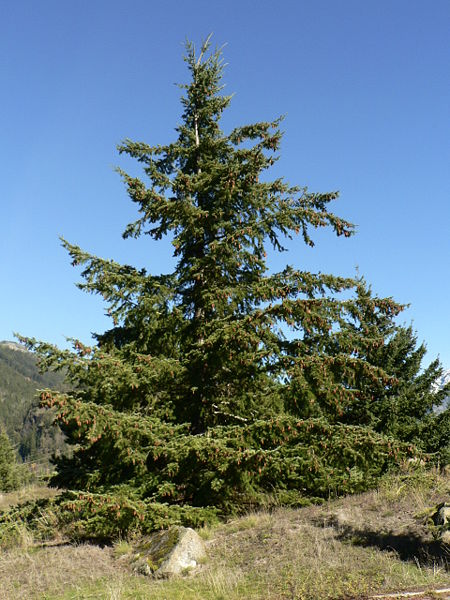
\includegraphics[keepaspectratio, width  =\textwidth]{img/doug-fir}\\
		\end{column}
		\begin{column}{0.6\textwidth}

\centering
The Douglas fir genome is 16Gbp long!\\
\vspace{20pt}

\textit{How many trees would you need to cut down to print out the Douglas fir genome?}\\
\vspace{20pt}
Single sided using MS Word default settings \\
\vspace{10pt}
						\centering	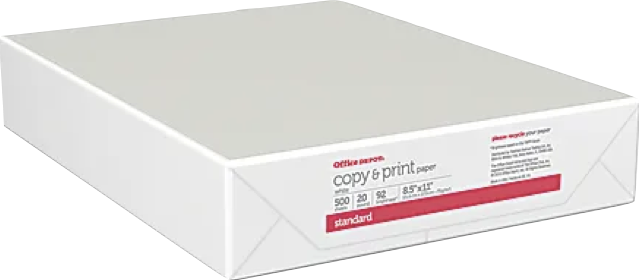
\includegraphics[keepaspectratio, width  =0.7\textwidth]{img/reamOpaper}\\

		\end{column}
	\end{columns}
\end{frame}


\begin{frame}
	\frametitle{Print Out the Douglas-fir Genome}
	\begin{columns}
		\begin{column}{0.4\textwidth}
			\centering	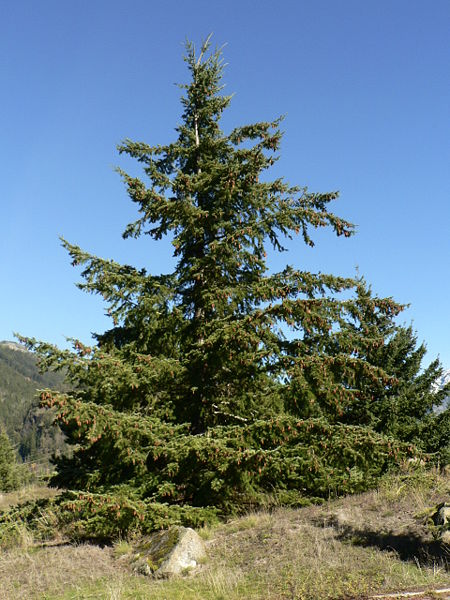
\includegraphics[keepaspectratio, width  =0.9\textwidth]{img/doug-fir}\\
			\vspace{5pt}
			\centering	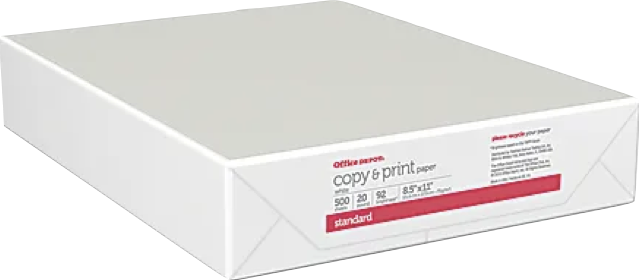
\includegraphics[keepaspectratio, width  =0.7\textwidth]{img/reamOpaper}\\
		\end{column}
		\begin{column}{0.6\textwidth}
			
			\centering \small 
			\begin{itemize}

		\item[--] The Douglas fir genome is approximately 16Gbp in size
		\item[--] With standard formatting a piece of paper (US Letter) would contain about 3,000 characters (As, Ts, Gs, Cs and Ns)

		\item[--] That gives a total of ($16 \times 10^9)/3000 = 5,333,333$ million sheets of paper
		\item[--] A single pine tree (45' trunk, 8" diameter) would give you about 10,000-20,000 sheets of paper
		\end{itemize}
			
		\end{column}
	\end{columns}
	\vspace{5pt}\pause
	\textbf{You would need to cut down about 360 trees to print it out}
	
\end{frame}

	
	
	
	\begin{frame}
		\frametitle{What Makes Conifer Genomes so Large?}
		\begin{columns}
			\begin{column}{0.7\textwidth}
				\small		
				\begin{itemize}
					\item[] Mobile DNA elements (aka jumping genes) can duplicate themselves in a host’s genome
					\item[] Similar life cycle to a virus
					\item[] Responsible for huge proportion of the repetitive DNA in eukaryotic genomes
				\end{itemize}
				\centering	\includegraphics[keepaspectratio, width  = 0.6\textwidth]{img/transposons.png}\\
			\end{column}
			\begin{column}{0.4\textwidth}
				\centering	\includegraphics[keepaspectratio, width  = \textwidth]{img/mcclintock}\\
				
			\end{column}
		\end{columns}
		\blfootnote{Transposable elements are truly fascinating! Figure from Liu and El-Kassaby 2019 \textit{Genes}}
	\end{frame}
	
	
	\begin{frame}
		
		\frametitle{The Douglas-fir genome}
		\small
		\begin{columns}
			\begin{column}{0.5\textwidth}
\textbf{					The first assembly of the Douglas-fir genome was published in 2017\\}
					\begin{itemize}

					\item[--] Primily based on short-read (151bp) technology
					\item[--] Assembed genome size of 14.95Gbp
					\item[--] N50 = 341kbp
					\item[--] 2.8 million assembled chunks
					
			\end{itemize}
			\end{column}
			\begin{column}{0.5\textwidth}
				\pause
				
\textbf{				UBC MSc student Meg Smith is currently (i.e. upstairs right now) re-assembling the Douglas-fir genome}
				
				\begin{itemize}
					\item[--] Primily based on long-read technology (median read length 15kbp) 
					\item[--] Assembed genome size of 15.21Gbp
					\item[--] N50 = 1.34Gbp
					\item[--] 3,012 assembled chunks
					
				\end{itemize}
			\end{column}
		\end{columns}
		
		\vspace{10pt}
\scriptsize	\textbf{Note:} This is not a criticism of the 2017 assembly, it's a statement on how rapidly the technilogy has moved on!
\blfootnote{N50 = at east half the assembled chunks are in chunks greater than or equal to this size. This number can be used to compare different genome assemblies}
	\end{frame}

	

		
	\begin{frame}
		
		\frametitle{The Douglas-fir genome}
		\small
		\begin{columns}
			\begin{column}{0.5\textwidth}
				\centering	\includegraphics[keepaspectratio, width  = \textwidth]{img/doug-fir}\\
							\end{column}
			\begin{column}{0.5\textwidth}
				
				The long-read based genome assembly of Douglas-fir is a vast improvement over the earlier, short-read based one. However, 
				\begin{itemize}
					\item[--] Repetitive DNA is still a \textbf{major }stumbling block for genomics
					\item[--] Understanding the genome is now a managable for Douglas-fir, but this does not make application of genomics straightforward

				\end{itemize}
			\end{column}
		\end{columns}
	\end{frame}
	
	%%% Slide 17 
	
	
	\begin{frame}
		\frametitle{Learning Outcomes}
		\begin{itemize}
			\item[--] Introduction to different sequencing methods
			\item[--] An introduction to genomics in conifers
			\item[--] The difficulty of repetitive DNA for genomic analysis
			\item[--] The pros and cons of different sequencing methods
		\end{itemize}
	\end{frame}


\begin{frame}
	\frametitle{A Thought For Next Time...}
	\Huge What are some uses for genomics in forestry?\\
	\vspace{20pt}
	\normalsize Think about how different aspects of conifer life history make the application of genetic and genomic technology difficult in conifers...
\end{frame}


		
\end{document}




